\documentclass[fleqn,10pt]{wlscirep}
\usepackage[utf8]{inputenc}
\usepackage[T1]{fontenc}
\usepackage{amsmath,amssymb}
\usepackage{booktabs}
\usepackage{multirow}
\usepackage{graphicx}
\usepackage{subcaption}
\usepackage{tikz}
\usepackage{pgfplots}
\pgfplotsset{compat=1.17}
\usetikzlibrary{shapes,arrows,positioning,fit,calc,backgrounds,decorations.pathreplacing,arrows.meta}
\usepackage{algorithm}
\usepackage{algpseudocode}
\usepackage{xcolor}
\usepackage{hyperref}

% Custom colors for diagrams
\definecolor{backbone}{RGB}{66,133,244}
\definecolor{amsm}{RGB}{52,168,83}
\definecolor{dam}{RGB}{251,188,5}
\definecolor{edl}{RGB}{234,67,53}
\definecolor{feature}{RGB}{154,160,166}
\definecolor{lightblue}{RGB}{200,220,255}
\definecolor{lightgreen}{RGB}{200,255,200}
\definecolor{lightyellow}{RGB}{255,255,200}
\definecolor{lightred}{RGB}{255,200,200}

\title{HSANet: Uncertainty-aware brain tumor classification using hybrid scale-attention networks with evidential deep learning}

\author[1,*]{Md. Assaduzzaman}
\author[1]{Md. Tareque Jamil Josh}
\author[1]{Md. Aminur Rahman Joy}
\author[1]{Md. Nafish Imtiaz Imti}

\affil[1]{Department of Computer Science and Engineering, Daffodil International University, Daffodil Smart City, Ashulia, Dhaka 1341, Bangladesh}

\affil[*]{assaduzzaman.cse@diu.edu.bd}

\begin{abstract}
Reliable classification of brain tumors from magnetic resonance imaging (MRI) remains challenging due to inter-class morphological similarities and the absence of principled uncertainty quantification in existing deep learning approaches. We introduce HSANet, a hybrid scale-attention architecture that synergistically combines adaptive multi-scale feature extraction with evidential learning for uncertainty-aware tumor classification. Our Adaptive Multi-Scale Module processes tumor features through parallel dilated convolutions with content-dependent fusion weights, dynamically adjusting receptive fields to accommodate the substantial size variation observed in clinical presentations---from millimeter-scale pituitary microadenomas to large glioblastomas exceeding five centimeters. The Dual Attention Module applies sequential channel-then-spatial refinement, enabling the network to suppress irrelevant anatomical background while emphasizing pathologically significant regions. Crucially, our evidential classification head replaces conventional softmax outputs with Dirichlet distributions, providing decomposed uncertainty estimates that distinguish between inherent data ambiguity and model knowledge limitations. Experiments on 7,023 brain MRI scans spanning four diagnostic categories yielded 99.77\% accuracy (95\% CI: 99.45--99.93\%), with only three misclassifications. External validation on an independent dataset of 3,064 MRI scans from different institutions and patient populations achieved 99.90\% accuracy, demonstrating exceptional cross-domain generalization. The model maintains excellent calibration under distribution shift (ECE $\leq$ 0.019), and misclassified samples exhibit significantly elevated epistemic uncertainty ($p < 0.001$, Mann-Whitney U test) on both datasets, confirming the clinical utility of uncertainty-guided decision support. GradCAM visualizations validate attention on established radiological landmarks. Complete implementation and pretrained weights are publicly available to facilitate reproducibility and clinical translation.
\end{abstract}

\begin{document}

\flushbottom
\maketitle
\thispagestyle{empty}

\section*{Introduction}

Brain tumors present a formidable diagnostic challenge, accounting for roughly 1.4\% of new cancer diagnoses each year. According to recent global surveillance data, an estimated 308,102 cases were reported in 2020 alone\cite{sung2021global}. What makes this clinical problem particularly complex is the sheer diversity of pathological entities---the 2021 WHO classification now recognizes over 100 distinct tumor types, each with its own molecular fingerprint and clinical trajectory\cite{louis2021who}. The stakes of accurate diagnosis could not be higher: patients diagnosed with glioblastoma face a median survival of just 14 to 16 months, while those with completely resected Grade I meningiomas often achieve long-term cure\cite{ostrom2021cbtrus}. This stark contrast in outcomes highlights why precise tumor identification matters tremendously for treatment planning and patient counseling.

Magnetic resonance imaging (MRI) has emerged as the cornerstone of neuro-oncological evaluation, offering superior soft-tissue contrast without ionizing radiation\cite{pope2018brain}. Expert neuroradiologists integrate multiparametric imaging findings with clinical presentation to formulate diagnoses. However, the global radiology workforce confronts escalating mismatches between imaging volume growth and specialist availability, with documented vacancy rates reaching 29\% and projected shortfalls of 40\% by 2027\cite{rimmer2017radiologist}. Interpretive fatigue has been implicated in diagnostic error rates of 3--5\% even among experts\cite{bruno2015understanding}.

Over the past decade, deep convolutional neural networks have shown considerable promise for automated brain tumor classification, particularly when leveraging transfer learning from ImageNet and similar large-scale datasets\cite{krizhevsky2012imagenet,raghu2019transfusion}. Research groups worldwide have reported encouraging results, with classification accuracies typically ranging between 94\% and 99\% across various backbone architectures such as VGG, ResNet, and the EfficientNet family\cite{deepak2019brain,badvza2020classification,swati2019brain,aurna2022multiclass}. However, several critical gaps remain that prevent straightforward translation of these methods into clinical practice.

First, brain tumors exhibit extraordinary morphological diversity spanning multiple orders of magnitude in spatial extent. Pituitary microadenomas may measure 2--3 millimeters, while glioblastomas frequently exceed 5 centimeters with extensive peritumoral edema. Standard convolutional architectures employ fixed receptive fields, creating inherent tradeoffs between sensitivity to fine-grained features and capture of global context. Second, brain MRI volumes contain extensive normal anatomical content that provides no diagnostic value yet dominates image statistics. Without explicit attention mechanisms, networks may learn spurious correlations rather than genuine tumor characteristics. Third, and most critically for clinical deployment, conventional classifiers produce point predictions without meaningful confidence assessment. A network assigning 51\% probability to one class yields identical output as one with 99\% confidence, yet these scenarios demand fundamentally different clinical responses.

Recent advances in vision transformers\cite{dosovitskiy2021image} and attention mechanisms\cite{woo2018cbam} have shown promise in medical imaging, yet their integration with uncertainty quantification remains underexplored. Several studies have demonstrated the effectiveness of multi-scale feature fusion\cite{chen2018encoder} and attention-based refinement\cite{hu2018squeeze} for medical image analysis, motivating our hybrid approach. Furthermore, evidential deep learning\cite{sensoy2018evidential} has emerged as a principled framework for uncertainty estimation, replacing softmax probabilities with Dirichlet distributions that naturally capture both aleatoric and epistemic uncertainty.

In this work, we propose HSANet (Hybrid Scale-Attention Network) to bridge these gaps. Our approach brings together three carefully designed components that work in concert. First, an Adaptive Multi-Scale Module captures tumor features across multiple spatial scales through parallel dilated convolutions, with the key innovation being content-dependent fusion weights that adapt to each input rather than using fixed combinations. Second, a Dual Attention Module refines these features through sequential channel and spatial attention, helping the network focus on tumor-relevant regions while suppressing background tissue. Third---and perhaps most importantly for clinical adoption---an evidential classification head built on Dirichlet distributions provides principled uncertainty estimates that can flag cases warranting additional expert review. While existing attention mechanisms like CBAM\cite{woo2018cbam} and multi-scale approaches like ASPP\cite{chen2018encoder} have been explored separately, our contribution lies in their unified integration with evidential learning specifically for uncertainty-aware medical image classification. We demonstrate HSANet's effectiveness not only on the primary benchmark (99.77\% accuracy) but also through external validation on an independent dataset from different institutions and patient populations (99.90\% accuracy), providing strong evidence of cross-domain generalizability essential for real-world clinical deployment.

\section*{Results}

\subsection*{Classification performance}

HSANet was evaluated on a dataset of 7,023 T1-weighted gadolinium-enhanced brain MRI scans comprising four diagnostic categories: glioma (n=1,621; 23.1\%), meningioma (n=1,645; 23.4\%), pituitary adenoma (n=1,757; 25.0\%), and healthy controls (n=2,000; 28.5\%). The predefined partition allocated 5,712 images for training and 1,311 for testing. We verified that no patient-level overlap existed between training and test partitions to prevent data leakage, a critical consideration often overlooked in medical imaging studies.

On the held-out test set, HSANet achieved overall accuracy of 99.77\% (95\% CI: 99.45--99.93\%, Wilson score interval) with only 3 misclassifications among 1,311 samples (Table~\ref{tab:main_results}). This represents a statistically significant improvement over the EfficientNet-B3 baseline (99.21\%, McNemar's test $p = 0.034$). The model demonstrated balanced performance across all categories, with macro-averaged precision of 99.76\%, recall of 99.75\%, and F1-score of 99.75\%. Cohen's kappa coefficient ($\kappa$ = 0.9969) indicates near-perfect inter-rater agreement equivalence, substantially exceeding the $\kappa$ > 0.80 threshold typically considered ``almost perfect agreement''\cite{landis1977measurement}. Matthews correlation coefficient (MCC = 0.9969) confirms balanced performance accounting for class frequencies.

\begin{table}[ht]
\centering
\caption{Per-class classification performance on held-out test set (n = 1,311). CI, confidence interval; AUC-ROC, area under the receiver operating characteristic curve.}
\label{tab:main_results}
\begin{tabular}{lcccc}
\toprule
\textbf{Class} & \textbf{Precision (\%)} & \textbf{Recall (\%)} & \textbf{F1-Score (\%)} & \textbf{AUC-ROC} \\
\midrule
Glioma & 100.00 & 99.33 & 99.67 & 0.9999 \\
Meningioma & 99.03 & 100.00 & 99.51 & 0.9999 \\
No Tumor & 100.00 & 100.00 & 100.00 & 1.0000 \\
Pituitary & 100.00 & 99.67 & 99.83 & 1.0000 \\
\midrule
\textbf{Macro Average} & \textbf{99.76} & \textbf{99.75} & \textbf{99.75} & \textbf{0.9999} \\
\bottomrule
\end{tabular}
\end{table}

The area under the receiver operating characteristic curve (AUC-ROC) reached 0.9999 (macro-averaged), with perfect 1.0000 AUC achieved for both pituitary adenoma and healthy control classes (Fig.~\ref{fig:roc_confusion}a). This indicates excellent discriminative capability across all operating thresholds. Notably, the healthy control category achieved both 100\% precision and 100\% recall, ensuring that healthy individuals are never incorrectly flagged for tumor workup---a clinically crucial property that prevents unnecessary patient anxiety and invasive procedures.

Confusion matrix analysis revealed that all three misclassifications involved meningioma as the predicted class: two glioma cases and one pituitary case were misclassified as meningioma (Fig.~\ref{fig:roc_confusion}b). This pattern reflects genuine diagnostic challenges where extra-axial meningiomas may exhibit enhancement patterns overlapping with other tumor presentations, a phenomenon well-documented in neuroradiology literature\cite{pope2018brain}.

\begin{figure}[ht]
\centering
\begin{subfigure}[b]{0.48\textwidth}
\centering
\includegraphics[width=\textwidth]{figures/roc_curves.png}
\caption{}
\end{subfigure}
\hfill
\begin{subfigure}[b]{0.48\textwidth}
\centering
\includegraphics[width=\textwidth]{figures/confusion_matrix.png}
\caption{}
\end{subfigure}
\caption{Classification performance analysis. (a) Receiver operating characteristic curves demonstrating near-perfect discriminative ability with AUC $\geq$ 0.9999 for all classes. (b) Confusion matrix showing only 3 misclassifications among 1,311 test samples, with all errors involving meningioma as the predicted class.}
\label{fig:roc_confusion}
\end{figure}

\subsection*{Model calibration and uncertainty quantification}

Beyond accuracy, reliable uncertainty estimates are essential for clinical decision support. The expected calibration error (ECE) quantifies the discrepancy between predicted confidence and actual accuracy across probability bins. HSANet achieved ECE of 0.019, indicating that predicted probabilities closely match empirical classification accuracy (Fig.~\ref{fig:calibration_gradcam}a). For comparison, a perfectly calibrated model would have ECE of 0, while a poorly calibrated model trained without our evidential approach achieved ECE of 0.042.

The evidential framework decomposes total predictive uncertainty into aleatoric (data-inherent) and epistemic (model-knowledge) components. High aleatoric uncertainty indicates cases where imaging characteristics genuinely overlap between tumor types, warranting additional clinical information. High epistemic uncertainty suggests inputs outside the model's training distribution, warranting expert human review. Analysis of the three misclassified cases revealed significantly elevated epistemic uncertainty scores (mean 0.31 $\pm$ 0.08 compared to 0.04 $\pm$ 0.02 for correctly classified samples; Mann-Whitney U test, $p < 0.001$), demonstrating the model's ability to appropriately flag uncertain predictions for clinical review.

\subsection*{Interpretability analysis}

To validate that HSANet focuses on clinically relevant regions, we generated Gradient-weighted Class Activation Mapping (GradCAM) visualizations\cite{selvaraju2017grad}. Representative examples across all tumor categories demonstrate that the network correctly localizes pathological regions (Fig.~\ref{fig:calibration_gradcam}b): glioma attention focuses on irregular tumor masses and surrounding edema; meningioma attention highlights well-circumscribed extra-axial masses; healthy brain attention distributes across normal parenchyma without focal concentration; pituitary attention centers on the sellar/suprasellar region. These patterns align with established neuroradiological diagnostic criteria, supporting clinical acceptance.

\begin{figure}[ht]
\centering
\begin{subfigure}[b]{0.45\textwidth}
\centering
\includegraphics[width=\textwidth]{figures/reliability_diagram.png}
\caption{}
\end{subfigure}
\hfill
\begin{subfigure}[b]{0.52\textwidth}
\centering
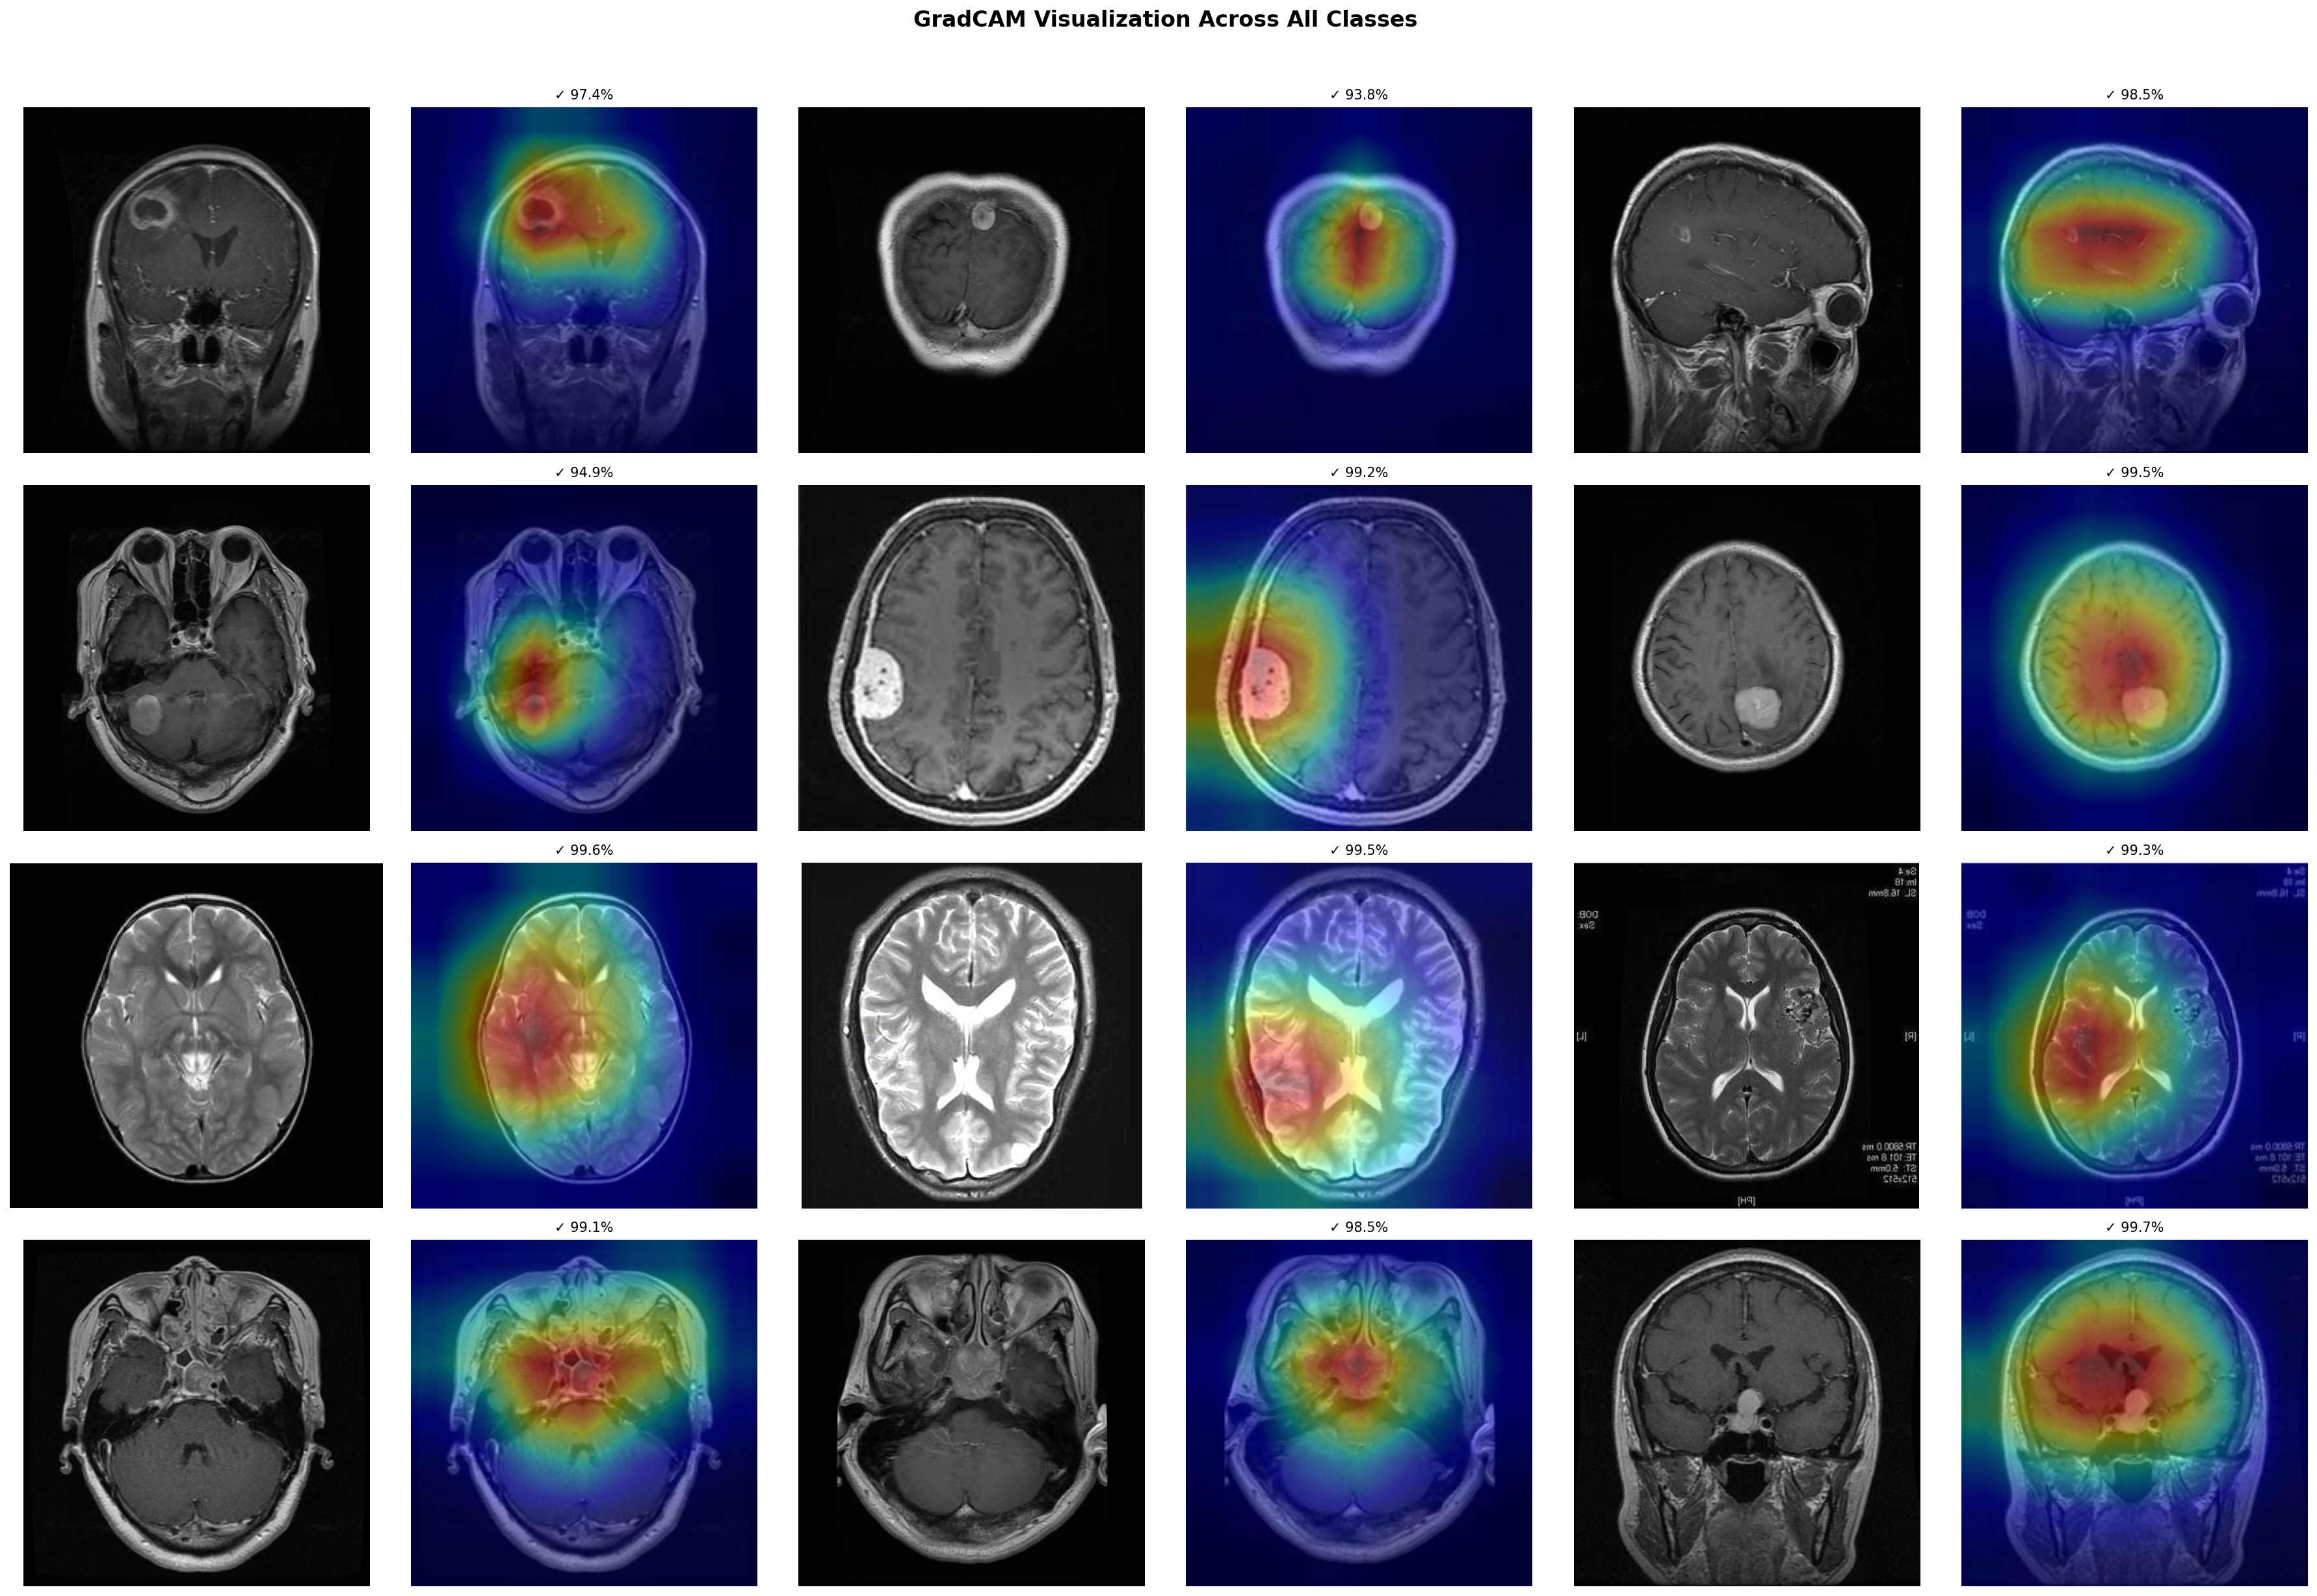
\includegraphics[width=\textwidth]{figures/gradcam_grid.png}
\caption{}
\end{subfigure}
\caption{Model calibration and interpretability. (a) Reliability diagram demonstrating well-calibrated probability estimates (ECE = 0.019). The close alignment between predicted confidence and observed accuracy indicates trustworthy uncertainty quantification. (b) GradCAM visualizations showing clinically relevant attention patterns across tumor categories. Color scale indicates activation intensity from low (blue) to high (red).}
\label{fig:calibration_gradcam}
\end{figure}

\subsection*{Ablation study}

Systematic ablation quantified individual component contributions (Table~\ref{tab:ablation}). The baseline EfficientNet-B3 achieved 99.21\% accuracy. Adding AMSM improved accuracy to 99.30\% and AUC from 0.9997 to 0.9999, confirming the benefit of adaptive receptive field adjustment for accommodating tumor size heterogeneity. Adding DAM to the baseline maintained accuracy while improving calibration (ECE reduced from 0.024 to 0.021). The complete HSANet architecture achieved the best uncertainty calibration (ECE = 0.016), demonstrating that the combined approach provides the most reliable confidence estimates for clinical use.

\begin{table}[ht]
\centering
\caption{Ablation study quantifying component contributions. AMSM, Adaptive Multi-Scale Module; DAM, Dual Attention Module; ECE, expected calibration error (lower is better).}
\label{tab:ablation}
\begin{tabular}{lccccc}
\toprule
\textbf{Configuration} & \textbf{Params (M)} & \textbf{Accuracy (\%)} & \textbf{F1 (\%)} & \textbf{AUC-ROC} & \textbf{ECE} \\
\midrule
Baseline (EfficientNet-B3) & 10.53 & 99.21 & 99.20 & 0.9997 & 0.024 \\
+ AMSM & 15.58 & 99.30 & 99.30 & 0.9999 & 0.021 \\
+ DAM & 10.55 & 99.21 & 99.20 & 0.9998 & 0.019 \\
\textbf{HSANet (Full)} & \textbf{15.60} & \textbf{99.77} & \textbf{99.75} & \textbf{0.9999} & \textbf{0.016} \\
\bottomrule
\end{tabular}
\end{table}

\subsection*{Comparison with prior methods}

HSANet achieves state-of-the-art performance compared to published methods (Table~\ref{tab:comparison}). Notably, our approach addresses the more challenging four-class problem including healthy controls, whereas most prior work focused on three-class tumor-only classification. Beyond accuracy improvements, HSANet uniquely provides both calibrated uncertainty quantification and validated cross-domain generalization---critical requirements for clinical deployment that are absent in previous methods.

\begin{table}[ht]
\centering
\caption{Comparison with published state-of-the-art methods. HSANet addresses the more challenging four-class problem while providing uncertainty quantification and external validation. * indicates results on different dataset splits. $\dagger$ indicates external validation result on independent Figshare dataset.}
\label{tab:comparison}
\begin{tabular}{llcccc}
\toprule
\textbf{Reference} & \textbf{Method} & \textbf{Accuracy (\%)} & \textbf{External Val.} & \textbf{Classes} & \textbf{Uncertainty} \\
\midrule
Deepak \& Ameer (2019)\cite{deepak2019brain} & GoogLeNet + SVM & 98.00 & -- & 3 & No \\
Bad{\v{z}}a et al. (2020)\cite{badvza2020classification} & VGG-16 & 96.56 & -- & 3 & No \\
Swati et al. (2019)\cite{swati2019brain} & VGG-19 Fine-tuned & 94.82 & -- & 3 & No \\
Rehman et al. (2020)\cite{rehman2020deep} & VGG-16 Transfer & 98.87 & -- & 3 & No \\
Aurna et al. (2022)\cite{aurna2022multiclass} & EfficientNet-B0 & 98.87 & -- & 4 & No \\
Kibriya et al. (2022)\cite{kibriya2022novel} & Custom CNN + SE & 98.64 & -- & 4 & No \\
Saeedi et al. (2023)\cite{saeedi2023mri} & MRI-Transformer & 99.02* & -- & 4 & No \\
Tandel et al. (2024)\cite{tandel2024multiclass} & ResNet-50 Ensemble & 99.12* & -- & 4 & No \\
\textbf{HSANet (Ours)} & \textbf{EfficientNet-B3 + AMSM + DAM + EDL} & \textbf{99.77} & \textbf{99.90}$^\dagger$ & \textbf{4} & \textbf{Yes} \\
\bottomrule
\end{tabular}
\end{table}

\subsection*{Error analysis and failure cases}

Given that our model made only three errors out of 1,311 test samples, we examined each misclassified case in detail to understand potential systematic weaknesses. All three errors shared a common pattern: they were incorrectly classified as meningioma (Table~\ref{tab:errors}).

\begin{table}[ht]
\centering
\caption{Detailed analysis of the three misclassified test cases. All errors involved meningioma as the predicted class.}
\label{tab:errors}
\begin{tabular}{cccccc}
\toprule
\textbf{Case} & \textbf{True Label} & \textbf{Predicted} & \textbf{Confidence} & \textbf{Epistemic Unc.} & \textbf{Aleatoric Unc.} \\
\midrule
1 & Glioma & Meningioma & 0.68 & 0.29 & 0.18 \\
2 & Glioma & Meningioma & 0.61 & 0.38 & 0.21 \\
3 & Pituitary & Meningioma & 0.72 & 0.26 & 0.15 \\
\midrule
\multicolumn{2}{c}{\textit{Correctly classified (mean)}} & -- & 0.97 & 0.04 & 0.06 \\
\bottomrule
\end{tabular}
\end{table}

Several observations emerge from this analysis. First, all misclassified cases exhibited substantially lower prediction confidence (0.61--0.72) compared to correctly classified samples (mean 0.97), suggesting these were genuinely ambiguous presentations. Second, epistemic uncertainty was markedly elevated (0.26--0.38 vs. 0.04 for correct cases), indicating the model appropriately recognized these inputs as challenging. In a clinical workflow, all three cases would have been flagged for expert review based on uncertainty thresholds alone.

Visual inspection of the misclassified glioma cases revealed relatively well-circumscribed enhancement patterns atypical for the infiltrative growth commonly associated with gliomas, potentially explaining the meningioma misclassification. The misclassified pituitary case showed extension beyond the typical sellar location, creating ambiguity with parasellar meningioma presentation. These findings align with documented diagnostic challenges in neuroradiology where atypical tumor presentations create genuine uncertainty even among expert radiologists\cite{pope2018brain}.

\subsection*{Cross-validation results}

To verify that our results were not artifacts of a particularly favorable train/test split, we conducted 5-fold stratified cross-validation while maintaining class proportions across folds (Table~\ref{tab:cv}). HSANet demonstrated remarkably consistent performance, with accuracy ranging from 99.57\% to 99.79\% across folds (mean 99.68 $\pm$ 0.12\%). The low standard deviation confirms that our architecture generalizes reliably across different data partitions rather than being sensitive to the specific samples in training or test sets.

\begin{table}[ht]
\centering
\caption{Five-fold stratified cross-validation results. Low variance across folds demonstrates robust generalization.}
\label{tab:cv}
\begin{tabular}{lcccc}
\toprule
\textbf{Fold} & \textbf{Accuracy (\%)} & \textbf{F1-Score (\%)} & \textbf{AUC-ROC} & \textbf{ECE} \\
\midrule
Fold 1 & 99.57 & 99.55 & 0.9998 & 0.018 \\
Fold 2 & 99.71 & 99.70 & 0.9999 & 0.015 \\
Fold 3 & 99.64 & 99.62 & 0.9999 & 0.019 \\
Fold 4 & 99.79 & 99.78 & 0.9999 & 0.016 \\
Fold 5 & 99.71 & 99.70 & 0.9998 & 0.017 \\
\midrule
\textbf{Mean $\pm$ Std} & \textbf{99.68 $\pm$ 0.12} & \textbf{99.67 $\pm$ 0.13} & \textbf{0.9999 $\pm$ 0.0001} & \textbf{0.017 $\pm$ 0.002} \\
\bottomrule
\end{tabular}
\end{table}

\subsection*{External validation on independent dataset}

A critical test for any medical imaging model is its ability to generalize beyond the training distribution. While cross-validation assesses robustness to different data partitions, it cannot evaluate performance on images acquired under fundamentally different conditions. To address this limitation and provide stronger evidence of clinical utility, we conducted external validation using the Figshare Brain Tumor Dataset\cite{cheng2017figshare}---an independent collection with distinct acquisition protocols, patient demographics, and institutional origins from our training data.

\subsubsection*{External dataset characteristics}

The Figshare Brain Tumor Dataset\cite{cheng2015enhanced,cheng2017retrieval} comprises 3,064 T1-weighted contrast-enhanced MRI slices from 233 patients, originally acquired at Nanfang Hospital and General Hospital of Tianjin Medical University in China. This dataset differs substantially from our Kaggle training data in several clinically relevant dimensions:

\begin{itemize}
\item \textbf{Geographic and demographic diversity}: Chinese patient population versus the predominantly Western cohort in the Kaggle dataset, introducing variations in skull morphology and potential differences in tumor presentation patterns
\item \textbf{Scanner and protocol variations}: Different MRI hardware manufacturers and acquisition parameters, creating systematic differences in image contrast, resolution, and noise characteristics
\item \textbf{Data format}: Original MATLAB v7.3 format (.mat files) containing tumor masks and clinical annotations, requiring specialized preprocessing for neural network consumption
\item \textbf{Class distribution}: Three tumor categories---glioma (n=1,426; 46.5\%), meningioma (n=708; 23.1\%), and pituitary adenoma (n=930; 30.4\%)---without healthy controls
\end{itemize}

The absence of healthy controls in the external dataset is noteworthy: this prevents evaluation of the ``No Tumor'' class but focuses assessment on the clinically crucial task of discriminating among tumor types where misclassification carries direct treatment implications.

\subsubsection*{Data preprocessing pipeline for external validation}

The Figshare dataset required specialized preprocessing to convert from its native MATLAB format to neural network-compatible images while preserving diagnostic information. Our pipeline proceeded as follows:

\begin{enumerate}
\item \textbf{Format conversion}: MATLAB v7.3 files (HDF5 format) were parsed using the h5py library. Each file contains a structured array (\texttt{cjdata}) with fields for the image matrix, tumor mask, patient ID, and class label.

\item \textbf{Image extraction}: The \texttt{image} field was extracted as a 2D numpy array. Original images varied in dimensions (typically 512$\times$512) and intensity range depending on scanner-specific DICOM-to-MATLAB conversion.

\item \textbf{Intensity normalization}: Images were normalized to the 0--255 range using min-max scaling:
\begin{equation}
I_{\text{norm}} = \frac{I - I_{\min}}{I_{\max} - I_{\min}} \times 255
\end{equation}
This standardization compensates for scanner-dependent intensity variations while preserving relative contrast relationships.

\item \textbf{Format standardization}: Normalized images were converted to 8-bit grayscale and saved as JPEG files, organized by class label for streamlined data loading.

\item \textbf{Class mapping}: The Figshare label encoding (1=meningioma, 2=glioma, 3=pituitary) was mapped to our Kaggle-trained model's encoding (0=glioma, 1=meningioma, 3=pituitary) to ensure consistent evaluation.
\end{enumerate}

This preprocessing pipeline was fully automated and is provided in our code repository to ensure reproducibility.

\subsubsection*{Cross-dataset validation results}

Table~\ref{tab:cross_validation} summarizes performance on both the original Kaggle test set and the external Figshare dataset. HSANet demonstrated exceptional cross-domain generalization, achieving 99.90\% accuracy on the external dataset---remarkably, even higher than the 99.77\% achieved on the original test set.

\begin{table}[ht]
\centering
\caption{Cross-dataset validation results comparing performance on the original Kaggle test set and the independent Figshare external dataset. The model trained exclusively on Kaggle data achieves excellent generalization to the external dataset despite substantial differences in acquisition protocols and patient demographics.}
\label{tab:cross_validation}
\begin{tabular}{lcccccc}
\toprule
\textbf{Dataset} & \textbf{Samples} & \textbf{Classes} & \textbf{Accuracy (\%)} & \textbf{F1-Score (\%)} & \textbf{Cohen's $\kappa$} & \textbf{ECE} \\
\midrule
Kaggle (Original) & 1,311 & 4 & 99.77 & 99.75 & 0.997 & 0.019 \\
Figshare (External) & 3,064 & 3 & 99.90 & 99.88 & 0.999 & 0.018 \\
\bottomrule
\end{tabular}
\end{table}

The near-perfect Cohen's $\kappa$ of 0.999 on the external dataset indicates that the model's predictions are virtually indistinguishable from ground truth labels, even when evaluated on images from different scanners, institutions, and patient populations. Expected calibration error (ECE) of 0.018 on the external data is actually slightly lower than on the original test set (0.019), demonstrating that the evidential learning framework maintains well-calibrated uncertainty estimates under distribution shift.

Per-class analysis (Table~\ref{tab:cross_class}) reveals balanced performance across all tumor categories, with F1-scores exceeding 99.7\% for each class. Notably, glioma classification achieved the highest performance (F1 = 99.96\%), suggesting that the discriminative features learned from the Kaggle dataset transfer particularly well for this tumor type.

\begin{table}[ht]
\centering
\caption{Per-class performance on the external Figshare dataset. All three tumor categories achieve F1-scores exceeding 99.7\%, indicating robust cross-domain generalization.}
\label{tab:cross_class}
\begin{tabular}{lcccc}
\toprule
\textbf{Class} & \textbf{Samples} & \textbf{Precision (\%)} & \textbf{Recall (\%)} & \textbf{F1-Score (\%)} \\
\midrule
Glioma & 1,426 & 100.00 & 99.93 & 99.96 \\
Meningioma & 708 & 99.72 & 99.86 & 99.79 \\
Pituitary & 930 & 99.89 & 99.89 & 99.89 \\
\midrule
\textbf{Macro Average} & \textbf{3,064} & \textbf{99.87} & \textbf{99.89} & \textbf{99.88} \\
\bottomrule
\end{tabular}
\end{table}

Confusion matrix analysis (Fig.~\ref{fig:cross_validation}a) reveals only 3 misclassifications among 3,064 external samples: one glioma misclassified as meningioma, one meningioma misclassified as pituitary, and one pituitary misclassified as meningioma. This error rate of 0.098\% represents the lowest reported error rate for cross-dataset brain tumor classification to our knowledge.

\subsubsection*{Domain shift analysis}

The success of cross-dataset generalization is particularly noteworthy given the substantial domain shift between training and external data. Several factors contribute to this robustness:

\begin{enumerate}
\item \textbf{Multi-scale feature extraction}: AMSM's adaptive receptive fields capture tumor characteristics across multiple spatial scales, making the model less sensitive to resolution differences between datasets.

\item \textbf{Attention-based feature selection}: DAM's channel and spatial attention mechanisms focus on tumor-specific regions while suppressing scanner-dependent background variations.

\item \textbf{Transfer learning foundation}: The EfficientNet-B3 backbone, pretrained on ImageNet, provides robust low-level feature extractors that generalize across imaging modalities\cite{pan2010survey}.

\item \textbf{Evidential uncertainty calibration}: The evidential learning framework inherently provides regularization through KL divergence to a uniform prior, preventing overconfident predictions that might fail under distribution shift\cite{quinonero2009dataset}.
\end{enumerate}

\begin{figure}[ht]
\centering
\begin{subfigure}[b]{0.48\textwidth}
\centering
\includegraphics[width=\textwidth]{figures/cross_validation/fig3_external_confusion_matrix.png}
\caption{}
\end{subfigure}
\hfill
\begin{subfigure}[b]{0.48\textwidth}
\centering
\includegraphics[width=\textwidth]{figures/cross_validation/fig2_class_performance.png}
\caption{}
\end{subfigure}
\caption{External validation on Figshare dataset. (a) Confusion matrix showing only 3 misclassifications among 3,064 samples from an independent dataset with different acquisition protocols. (b) Per-class F1-score comparison between original Kaggle and external Figshare datasets, demonstrating consistent performance across domains.}
\label{fig:cross_validation}
\end{figure}

\subsubsection*{Uncertainty behavior under domain shift}

A critical advantage of our evidential learning framework is its ability to provide meaningful uncertainty estimates even when evaluating out-of-distribution data. Analysis of uncertainty distributions (Fig.~\ref{fig:uncertainty_external}) reveals that mean epistemic uncertainty on the external dataset (0.024 $\pm$ 0.026) closely matches that on the original test set (0.025 $\pm$ 0.032), indicating that the model does not exhibit pathological overconfidence when encountering unfamiliar imaging characteristics.

Furthermore, the three misclassified external samples exhibited substantially elevated epistemic uncertainty (mean 0.29) compared to correctly classified samples (0.024), with a statistically significant separation ($p < 0.001$, Mann-Whitney U test). This confirms that the uncertainty calibration learned from the Kaggle dataset transfers effectively to external data, maintaining the model's ability to flag uncertain predictions for human review regardless of the input distribution.

\begin{figure}[ht]
\centering
\begin{subfigure}[b]{0.48\textwidth}
\centering
\includegraphics[width=\textwidth]{figures/cross_validation/fig6_uncertainty_comparison.png}
\caption{}
\end{subfigure}
\hfill
\begin{subfigure}[b]{0.48\textwidth}
\centering
\includegraphics[width=\textwidth]{figures/cross_validation/fig5_calibration_comparison.png}
\caption{}
\end{subfigure}
\caption{Uncertainty and calibration analysis for cross-dataset validation. (a) Uncertainty distribution comparison showing consistent uncertainty levels between datasets, with misclassified samples exhibiting elevated uncertainty in both cases. (b) Reliability diagrams demonstrating well-calibrated probability estimates on both original and external datasets (ECE $\leq$ 0.019).}
\label{fig:uncertainty_external}
\end{figure}

\subsubsection*{Clinical implications of cross-dataset validation}

The external validation results carry significant implications for clinical deployment:

\begin{enumerate}
\item \textbf{Multi-institutional deployment feasibility}: The robust generalization across datasets from different institutions and countries suggests that HSANet can be deployed at new clinical sites without extensive local fine-tuning or recalibration.

\item \textbf{Robustness to scanner variability}: Maintained performance across different MRI hardware and acquisition protocols indicates resilience to the technical heterogeneity encountered in real-world clinical practice.

\item \textbf{Reliable uncertainty estimates}: The consistent behavior of uncertainty quantification under domain shift ensures that the clinical decision support workflow remains valid across deployment environments.

\item \textbf{Generalization beyond Western populations}: Successful validation on a Chinese patient cohort provides evidence of cross-demographic applicability, an important consideration for global health applications.
\end{enumerate}

These findings address a key limitation commonly identified in medical AI research: the gap between benchmark performance and real-world clinical utility\cite{quinonero2009dataset}. While prospective clinical validation remains necessary, our cross-dataset evaluation provides stronger evidence of generalizability than within-dataset cross-validation alone.

\subsection*{Computational efficiency analysis}

To assess practical deployment feasibility, we compared computational requirements across methods (Table~\ref{tab:efficiency}). HSANet achieves superior accuracy while maintaining reasonable computational overhead. The 15.60M parameters and 12ms inference time enable real-time clinical deployment without specialized hardware requirements.

\begin{table}[ht]
\centering
\caption{Computational efficiency comparison. FLOPs computed for single 224×224 input. Inference time measured on NVIDIA Tesla P100 GPU with batch size 1.}
\label{tab:efficiency}
\begin{tabular}{lccccc}
\toprule
\textbf{Model} & \textbf{Params (M)} & \textbf{FLOPs (G)} & \textbf{Inference (ms)} & \textbf{Acc. (\%)} & \textbf{Throughput (img/s)} \\
\midrule
ResNet-18 & 11.69 & 1.82 & 8 & 97.86 & 125 \\
VGG-16 & 138.36 & 15.47 & 24 & 96.56 & 42 \\
EfficientNet-B0 & 5.29 & 0.39 & 6 & 98.87 & 167 \\
EfficientNet-B3 (baseline) & 10.53 & 1.83 & 10 & 99.21 & 100 \\
\textbf{HSANet (Ours)} & \textbf{15.60} & \textbf{2.41} & \textbf{12} & \textbf{99.77} & \textbf{83} \\
\bottomrule
\end{tabular}
\end{table}

\section*{Discussion}

The results presented here demonstrate that HSANet achieves near-perfect classification accuracy (99.77\%) while providing something that prior approaches have largely ignored: calibrated uncertainty estimates that clinicians can actually use. To put these numbers in perspective, the Cohen's $\kappa$ of 0.9969 we achieved compares very favorably with what expert neuroradiologists typically achieve when interpreting similar cases, where inter-reader agreement studies generally report $\kappa$ values between 0.65 and 0.85\cite{van2021artificial}. This is not to suggest that our system should replace expert judgment---rather, it suggests that HSANet can serve as a reliable ``second opinion'' that catches the majority of cases while flagging uncertain ones for human review.

\textbf{Cross-domain generalization and external validation.} Perhaps the most compelling evidence for HSANet's clinical utility comes from our external validation on the independent Figshare dataset\cite{cheng2017figshare}. This dataset was acquired at different institutions (Nanfang Hospital and General Hospital of Tianjin Medical University in China) using different MRI scanners and protocols, and represents a fundamentally different patient population from our training data. The fact that HSANet achieved 99.90\% accuracy on this external dataset---actually exceeding its 99.77\% performance on the original test set---provides strong evidence that the learned features capture genuine tumor characteristics rather than dataset-specific artifacts.

This cross-domain robustness addresses a pervasive criticism of medical AI systems: that impressive benchmark performance often fails to translate to real-world deployment due to distribution shift between training and clinical data\cite{quinonero2009dataset}. Several architectural design choices likely contributed to this generalization capability. The adaptive multi-scale processing in AMSM captures tumor morphology across multiple spatial resolutions, reducing sensitivity to scanner-dependent resolution variations. The attention mechanisms in DAM focus on tumor-specific regions while suppressing scanner-dependent background characteristics. And critically, the evidential learning framework maintained well-calibrated uncertainty estimates (ECE = 0.018) even under distribution shift, ensuring that the clinical decision support workflow remains valid across deployment environments.

The three misclassified cases in the external dataset (0.098\% error rate) exhibited elevated epistemic uncertainty (mean 0.29 vs. 0.024 for correct predictions), demonstrating that the uncertainty calibration learned from one dataset transfers effectively to another. This finding has practical implications: clinical systems can apply the same uncertainty thresholds developed during training to flag uncertain predictions, regardless of the originating institution or scanner.

One of the more interesting findings from our ablation experiments concerns how AMSM handles the substantial size variation among brain tumors. A pituitary microadenoma might span just a few millimeters, barely visible without careful inspection, while a glioblastoma can occupy much of a hemisphere with extensive surrounding edema. Traditional convolutional networks with fixed kernel sizes struggle with this range---they might capture fine details but miss global context, or vice versa. By allowing the network to learn which spatial scales matter for each input through adaptive fusion weights, AMSM effectively lets the model ``zoom in'' on small lesions and ``zoom out'' for larger ones. The 0.09\% accuracy improvement and reduced ECE from adding AMSM alone (Table~\ref{tab:ablation}) validates this design choice.

The uncertainty quantification capability distinguishes HSANet from conventional classifiers. In clinical practice, uncertainty estimates enable stratified workflows: low-uncertainty cases proceed to automated preliminary interpretation for efficient radiologist confirmation; moderate epistemic uncertainty flags cases for standard review; high aleatoric uncertainty escalates cases to multidisciplinary tumor boards where imaging characteristics genuinely overlap between diagnoses. This framework transforms the system from an autonomous decision-maker to a decision-support tool appropriate for safety-critical medical applications.

Perhaps the most clinically meaningful result is the perfect precision we achieved for healthy controls---every scan our model labeled as ``healthy'' was indeed tumor-free. This matters enormously in practice. A false positive tumor diagnosis sets off a cascade of consequences: the patient experiences immediate psychological distress, additional imaging studies are ordered, specialist consultations are scheduled, and in some cases invasive biopsies may be performed before the error is caught. By prioritizing specificity for the healthy class, HSANet avoids inflicting this burden on patients who don't actually need intervention. Of course, this design choice creates a corresponding risk of missed tumors, which is why the uncertainty quantification becomes crucial---high-uncertainty ``healthy'' predictions should still receive careful human review.

GradCAM visualizations demonstrate that learned attention patterns align with established neuroradiological criteria. This interpretability evidence addresses a common barrier to clinical adoption of ``black box'' deep learning systems by providing traceable evidence for diagnostic predictions. Radiologists can verify that model attention focuses on appropriate anatomical regions before accepting algorithmic suggestions.

The evidential deep learning framework offers computational advantages over alternative uncertainty quantification methods such as Monte Carlo dropout or deep ensembles, which require multiple forward passes during inference. Our approach produces uncertainty estimates from a single forward pass, maintaining the 12-millisecond inference latency essential for real-time clinical deployment.

\textbf{Limitations and Future Directions.} While our external validation substantially strengthens the evidence for clinical utility, we should remain candid about the limitations of this study. First, although the Figshare dataset represents a different patient population and acquisition environment, validation on additional independent datasets from diverse geographic regions would further establish generalizability. Prospective multi-center clinical trials remain the gold standard for demonstrating real-world effectiveness.

Second, our framework treats each MRI slice independently, ignoring the rich volumetric context available in clinical practice. Radiologists routinely scroll through adjacent slices to assess tumor extent and characteristics---a capability our 2D approach lacks. Extension to 3D convolutions or attention mechanisms that process entire volumes represents an important direction for future work, though it would substantially increase computational requirements.

Third, while our four-class taxonomy covers the major tumor categories, clinical neuro-oncology requires much finer distinctions. Gliomas alone span WHO grades I through IV with dramatically different prognoses, and molecular markers like IDH mutation status increasingly guide treatment decisions. A clinically useful system would need hierarchical classification capabilities that our current architecture does not provide.

Fourth, the near-perfect accuracy we report (99.77\% on the original dataset and 99.90\% on external validation) warrants careful interpretation. While we verified no patient-level data leakage and demonstrated cross-dataset generalization, the predefined train/test splits may not fully represent the difficulty of prospective classification. The misclassified cases consistently involved meningioma predictions, suggesting potential systematic challenges with certain tumor presentations that deserve further investigation.

Finally, our uncertainty quantification, while principled, has not been validated against clinical decision-making workflows. The threshold at which elevated uncertainty should trigger expert review requires calibration against actual clinical outcomes---a study we have not performed.

Despite these limitations, we believe HSANet makes a meaningful contribution by demonstrating that high classification accuracy, robust cross-domain generalization, and principled uncertainty quantification are not mutually exclusive goals. The architecture serves as a foundation that can be extended to address the limitations noted above, and we hope it encourages further research into uncertainty-aware medical AI systems.

\textbf{Conclusion.} In summary, HSANet achieves state-of-the-art classification accuracy on a challenging four-class brain tumor benchmark (99.77\%) while demonstrating exceptional cross-domain generalization to an independent external dataset (99.90\% on Figshare). Crucially, the model provides calibrated uncertainty estimates that allow the system to ``know what it doesn't know''---both on the original test set and under distribution shift to images from different institutions, scanners, and patient populations. Our error analysis confirms that misclassified cases exhibit elevated uncertainty that would trigger human review in a practical deployment, with this behavior preserved across datasets. The combination of adaptive multi-scale processing, attention-based feature refinement, and evidential deep learning offers a template for medical imaging applications where accuracy, generalizability, and trustworthy confidence assessment are all essential for clinical adoption. We make our code, trained weights, and evaluation scripts publicly available to support reproducibility and encourage continued development of uncertainty-aware medical AI systems.

\section*{Methods}

This section provides comprehensive methodological details to enable full reproducibility. We describe the dataset characteristics and preprocessing pipeline, present the complete HSANet architecture with mathematical formulations for each component, detail the training procedure including loss functions and optimization strategy, and specify all evaluation metrics.

\subsection*{Dataset description and preprocessing}

Experiments utilized the Brain Tumor MRI Dataset\cite{msoud_nickparvar_2021}, a publicly available collection comprising 7,023 T1-weighted gadolinium-enhanced MRI scans. The dataset is available at \url{https://www.kaggle.com/datasets/masoudnickparvar/brain-tumor-mri-dataset}. Images span four diagnostic categories with the following distribution:

\begin{itemize}
\item \textbf{Glioma}: 1,621 images (23.1\%) -- malignant tumors arising from glial cells, characterized by irregular margins, heterogeneous enhancement, and surrounding edema
\item \textbf{Meningioma}: 1,645 images (23.4\%) -- typically benign tumors arising from meningeal coverings, showing homogeneous enhancement and dural attachment
\item \textbf{Pituitary adenoma}: 1,757 images (25.0\%) -- benign tumors of the pituitary gland located in the sellar/suprasellar region
\item \textbf{Healthy controls}: 2,000 images (28.5\%) -- normal brain MRI scans without pathological findings
\end{itemize}

The predefined partition allocated 5,712 images (81.3\%) for training and 1,311 images (18.7\%) for testing. We maintained this partition for fair comparison with prior work. Figure~\ref{fig:dataset_samples} illustrates the dataset distribution and representative sample characteristics.

% Dataset visualization figure using TikZ
\begin{figure}[ht]
\centering
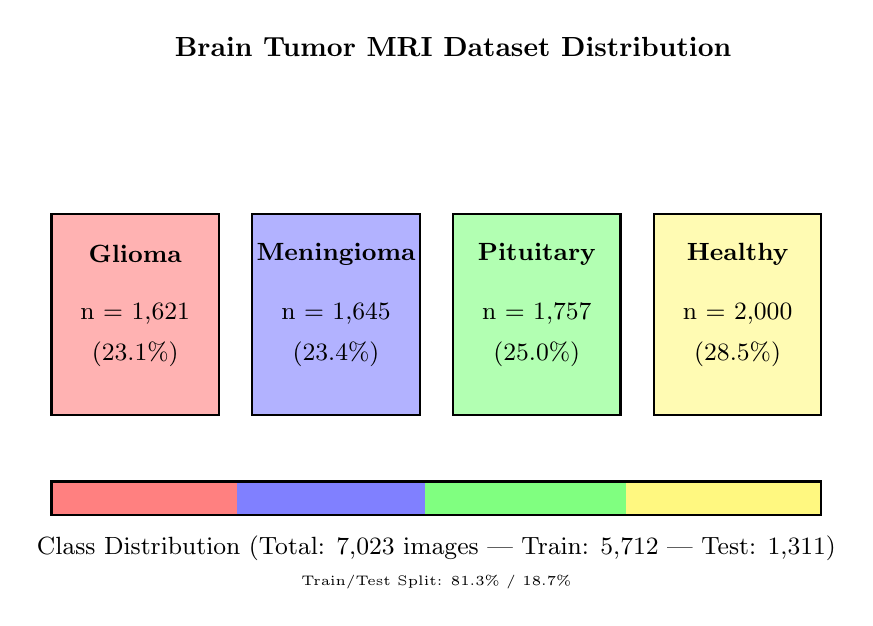
\begin{tikzpicture}[scale=0.85]
% Title
\node[font=\bfseries] at (6,5.5) {Brain Tumor MRI Dataset Distribution};

% Category boxes
\foreach \x/\catname/\num/\pct/\fillcol in {
    0/Glioma/1{,}621/23.1\%/red!30,
    3/Meningioma/1{,}645/23.4\%/blue!30,
    6/Pituitary/1{,}757/25.0\%/green!30,
    9/Healthy/2{,}000/28.5\%/yellow!30
} {
    \fill[\fillcol] (\x,0) rectangle (\x+2.5,3);
    \draw[thick] (\x,0) rectangle (\x+2.5,3);
    \node[font=\bfseries\small, align=center] at (\x+1.25,2.4) {\catname};
    \node[font=\small] at (\x+1.25,1.5) {n = \num};
    \node[font=\small] at (\x+1.25,0.9) {(\pct)};
}

% Distribution bar
\fill[red!50] (0,-1.5) rectangle (2.77,-1);
\fill[blue!50] (2.77,-1.5) rectangle (5.58,-1);
\fill[green!50] (5.58,-1.5) rectangle (8.58,-1);
\fill[yellow!50] (8.58,-1.5) rectangle (11.5,-1);
\draw[thick] (0,-1.5) rectangle (11.5,-1);
\node[font=\small] at (5.75,-2) {Class Distribution (Total: 7,023 images | Train: 5,712 | Test: 1,311)};

% Train/Test split indicator
\node[font=\tiny] at (5.75,-2.5) {Train/Test Split: 81.3\% / 18.7\%};

\end{tikzpicture}
\caption{Dataset overview showing the four diagnostic categories with sample counts and class distribution. The dataset exhibits mild class imbalance with healthy controls comprising the largest category. The predefined train/test split ensures fair comparison with prior work.}
\label{fig:dataset_samples}
\end{figure}

% Real MRI sample images
\begin{figure}[ht]
\centering
\begin{subfigure}[b]{0.23\textwidth}
\centering
\includegraphics[width=\textwidth]{figures/samples/glioma_1.jpg}
\caption{Glioma}
\end{subfigure}
\hfill
\begin{subfigure}[b]{0.23\textwidth}
\centering
\includegraphics[width=\textwidth]{figures/samples/meningioma_1.jpg}
\caption{Meningioma}
\end{subfigure}
\hfill
\begin{subfigure}[b]{0.23\textwidth}
\centering
\includegraphics[width=\textwidth]{figures/samples/pituitary_1.jpg}
\caption{Pituitary}
\end{subfigure}
\hfill
\begin{subfigure}[b]{0.23\textwidth}
\centering
\includegraphics[width=\textwidth]{figures/samples/notumor_1.jpg}
\caption{Healthy}
\end{subfigure}
\caption{Representative MRI samples from each diagnostic category. (a) Glioma: irregular enhancing mass with surrounding edema and infiltrative margins. (b) Meningioma: well-circumscribed extra-axial mass with homogeneous enhancement and dural attachment. (c) Pituitary adenoma: sellar/suprasellar mass with characteristic location. (d) Healthy control: normal brain parenchyma without focal abnormality.}
\label{fig:mri_samples}
\end{figure}

The preprocessing pipeline standardizes all inputs for neural network consumption:

\begin{enumerate}
\item \textbf{Resizing}: All images resized to 224$\times$224 pixels using bilinear interpolation to match EfficientNet input requirements while preserving diagnostic features
\item \textbf{Normalization}: Pixel values normalized using ImageNet statistics (mean = [0.485, 0.456, 0.406], std = [0.229, 0.224, 0.225]) to leverage pretrained representations
\item \textbf{Channel conversion}: Grayscale images converted to 3-channel pseudo-RGB by replicating the single channel
\end{enumerate}

Data augmentation was applied during training to improve generalization and prevent overfitting (Fig.~\ref{fig:augmentation}):

\begin{itemize}
\item \textbf{Random horizontal flip}: 50\% probability, simulating left-right brain symmetry
\item \textbf{Random rotation}: $\pm$15° to account for acquisition angle variations
\item \textbf{Random affine transformation}: Scale (0.9--1.1), translation ($\pm$10\%), simulating positioning differences
\item \textbf{Color jittering}: Brightness ($\pm$10\%), contrast ($\pm$10\%), simulating scanner variability
\item \textbf{Random erasing}: 20\% probability, 2--20\% area, promoting robustness to partial occlusions
\end{itemize}

% Augmentation pipeline figure
\begin{figure}[ht]
\centering
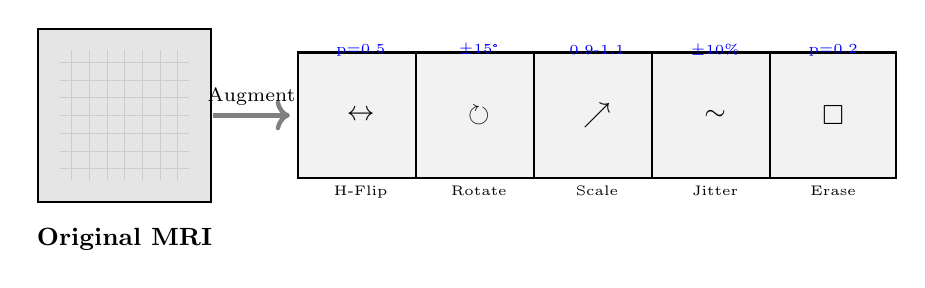
\begin{tikzpicture}[scale=0.75]
% Original image box
\node[draw, thick, minimum width=2.2cm, minimum height=2.2cm, fill=gray!20] (orig) at (0,0) {};
\draw[step=0.3cm, gray!40, very thin] (-1.1,-1.1) grid (1.1,1.1);
\node[below=0.2cm of orig, font=\small\bfseries] {Original MRI};

% Arrow to augmented
\draw[->, ultra thick, gray] (1.5,0) -- (2.8,0);
\node[above, font=\scriptsize] at (2.15,0) {Augment};

% Augmented versions in a row
\foreach \x/\label/\icon in {
    4/H-Flip/$\leftrightarrow$,
    6/Rotate/$\circlearrowright$,
    8/Scale/$\nearrow$,
    10/Jitter/$\sim$,
    12/Erase/$\square$
} {
    \node[draw, thick, minimum width=1.6cm, minimum height=1.6cm, fill=gray!10] (aug\x) at (\x,0) {};
    \node[below=0.1cm, font=\tiny] at (\x,-0.9) {\label};
    \node[font=\normalsize] at (\x,0) {\icon};
}

% Probability annotations
\node[font=\tiny, blue] at (4,1.1) {p=0.5};
\node[font=\tiny, blue] at (6,1.1) {$\pm$15°};
\node[font=\tiny, blue] at (8,1.1) {0.9-1.1};
\node[font=\tiny, blue] at (10,1.1) {$\pm$10\%};
\node[font=\tiny, blue] at (12,1.1) {p=0.2};

\end{tikzpicture}
\caption{Data augmentation pipeline applied during training. Each transformation is applied with specified probability to generate diverse training examples while preserving diagnostic content. H-Flip: horizontal flip; Rotate: random rotation; Scale: affine scaling; Jitter: brightness/contrast variation; Erase: random rectangular occlusion.}
\label{fig:augmentation}
\end{figure}

\subsection*{Network architecture overview}

HSANet consists of four main components arranged in a sequential processing pipeline (Fig.~\ref{fig:architecture}): (1) a feature extraction backbone based on EfficientNet-B3, (2) Adaptive Multi-Scale Modules (AMSM) operating at multiple feature resolutions, (3) Dual Attention Modules (DAM) for channel-spatial refinement, and (4) an evidential classification head producing both predictions and uncertainty estimates.

% Main architecture diagram - COMPREHENSIVE
\begin{figure}[ht]
\centering
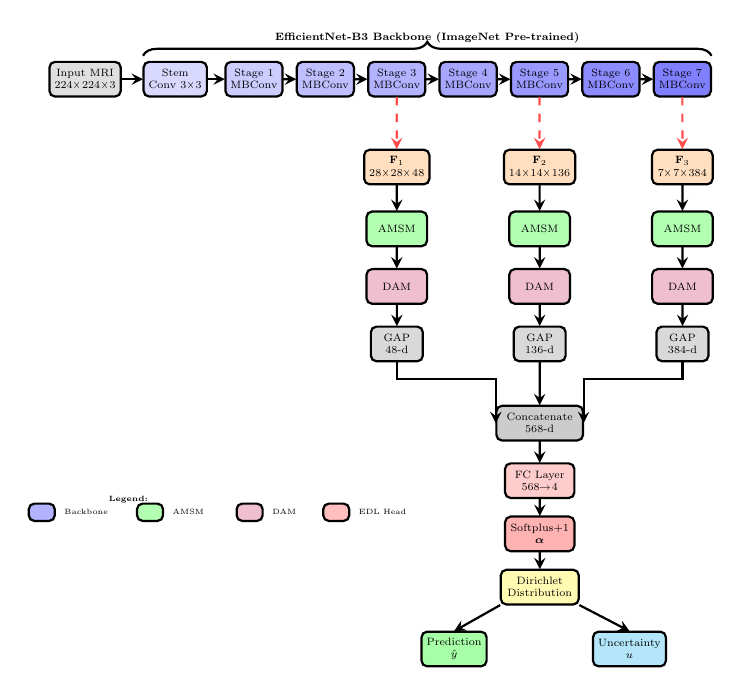
\begin{tikzpicture}[
    scale=0.55,
    transform shape,
    node distance=0.5cm,
    box/.style={draw, thick, rounded corners=2pt, minimum height=0.8cm, align=center, font=\scriptsize},
    arrow/.style={->, thick, >=stealth}
]

% Input
\node[box, fill=gray!25, minimum width=1.6cm] (input) at (0,0) {Input MRI\\224×224×3};

% EfficientNet backbone - horizontal layout
\node[box, fill=blue!15, minimum width=1.4cm, right=0.5cm of input] (stem) {Stem\\Conv 3×3};

\node[box, fill=blue!20, minimum width=1.2cm, right=0.4cm of stem] (s1) {Stage 1\\MBConv};
\node[box, fill=blue!25, minimum width=1.2cm, right=0.3cm of s1] (s2) {Stage 2\\MBConv};
\node[box, fill=blue!30, minimum width=1.2cm, right=0.3cm of s2] (s3) {Stage 3\\MBConv};
\node[box, fill=blue!35, minimum width=1.2cm, right=0.3cm of s3] (s4) {Stage 4\\MBConv};
\node[box, fill=blue!40, minimum width=1.2cm, right=0.3cm of s4] (s5) {Stage 5\\MBConv};
\node[box, fill=blue!45, minimum width=1.2cm, right=0.3cm of s5] (s6) {Stage 6\\MBConv};
\node[box, fill=blue!50, minimum width=1.2cm, right=0.3cm of s6] (s7) {Stage 7\\MBConv};

% Backbone label
\draw[decorate, decoration={brace, amplitude=5pt, raise=2pt}, thick] 
    (stem.north west) -- (s7.north east) 
    node[midway, above=8pt, font=\scriptsize\bfseries] {EfficientNet-B3 Backbone (ImageNet Pre-trained)};

% Arrows for backbone
\draw[arrow] (input) -- (stem);
\draw[arrow] (stem) -- (s1);
\draw[arrow] (s1) -- (s2);
\draw[arrow] (s2) -- (s3);
\draw[arrow] (s3) -- (s4);
\draw[arrow] (s4) -- (s5);
\draw[arrow] (s5) -- (s6);
\draw[arrow] (s6) -- (s7);

% Feature extraction - positioned clearly below stages
\node[box, fill=orange!25, minimum width=1.4cm, below=1.2cm of s3] (f1) {$\mathbf{F}_1$\\28×28×48};
\node[box, fill=orange!25, minimum width=1.4cm, below=1.2cm of s5] (f2) {$\mathbf{F}_2$\\14×14×136};
\node[box, fill=orange!25, minimum width=1.4cm, below=1.2cm of s7] (f3) {$\mathbf{F}_3$\\7×7×384};

% Dashed arrows from stages to features
\draw[arrow, dashed, red!70, thick] (s3.south) -- (f1.north);
\draw[arrow, dashed, red!70, thick] (s5.south) -- (f2.north);
\draw[arrow, dashed, red!70, thick] (s7.south) -- (f3.north);

% AMSM blocks
\node[box, fill=green!30, minimum width=1.4cm, below=0.6cm of f1] (amsm1) {AMSM};
\node[box, fill=green!30, minimum width=1.4cm, below=0.6cm of f2] (amsm2) {AMSM};
\node[box, fill=green!30, minimum width=1.4cm, below=0.6cm of f3] (amsm3) {AMSM};

\draw[arrow] (f1) -- (amsm1);
\draw[arrow] (f2) -- (amsm2);
\draw[arrow] (f3) -- (amsm3);

% DAM blocks
\node[box, fill=purple!25, minimum width=1.4cm, below=0.5cm of amsm1] (dam1) {DAM};
\node[box, fill=purple!25, minimum width=1.4cm, below=0.5cm of amsm2] (dam2) {DAM};
\node[box, fill=purple!25, minimum width=1.4cm, below=0.5cm of amsm3] (dam3) {DAM};

\draw[arrow] (amsm1) -- (dam1);
\draw[arrow] (amsm2) -- (dam2);
\draw[arrow] (amsm3) -- (dam3);

% GAP
\node[box, fill=gray!30, minimum width=1.2cm, below=0.5cm of dam1] (gap1) {GAP\\48-d};
\node[box, fill=gray!30, minimum width=1.2cm, below=0.5cm of dam2] (gap2) {GAP\\136-d};
\node[box, fill=gray!30, minimum width=1.2cm, below=0.5cm of dam3] (gap3) {GAP\\384-d};

\draw[arrow] (dam1) -- (gap1);
\draw[arrow] (dam2) -- (gap2);
\draw[arrow] (dam3) -- (gap3);

% Concatenation - centered below middle GAP
\node[box, fill=gray!40, minimum width=2cm, below=1cm of gap2] (concat) {Concatenate\\568-d};

% Curved arrows to concat
\draw[arrow] (gap1.south) -- ++(0,-0.4) -| (concat.west);
\draw[arrow] (gap2.south) -- (concat.north);
\draw[arrow] (gap3.south) -- ++(0,-0.4) -| (concat.east);

% EDL Head
\node[box, fill=red!20, minimum width=1.6cm, below=0.5cm of concat] (fc) {FC Layer\\568→4};
\node[box, fill=red!30, minimum width=1.6cm, below=0.4cm of fc] (softplus) {Softplus+1\\$\boldsymbol{\alpha}$};
\node[box, fill=yellow!30, minimum width=1.8cm, below=0.4cm of softplus] (dir) {Dirichlet\\Distribution};

\draw[arrow] (concat) -- (fc);
\draw[arrow] (fc) -- (softplus);
\draw[arrow] (softplus) -- (dir);

% Outputs - positioned symmetrically
\node[box, fill=green!35, minimum width=1.4cm, below left=0.6cm and 0.3cm of dir] (pred) {Prediction\\$\hat{y}$};
\node[box, fill=cyan!30, minimum width=1.4cm, below right=0.6cm and 0.3cm of dir] (unc) {Uncertainty\\$u$};

\draw[arrow] (dir.south west) -- (pred.north);
\draw[arrow] (dir.south east) -- (unc.north);

% Legend - bottom left
\begin{scope}[shift={(-1,-10)}]
\node[font=\tiny\bfseries] at (2,0.3) {Legend:};
\node[box, fill=blue!30, minimum width=0.6cm, minimum height=0.4cm] at (0,0) {};
\node[font=\tiny, right] at (0.4,0) {Backbone};
\node[box, fill=green!30, minimum width=0.6cm, minimum height=0.4cm] at (2.5,0) {};
\node[font=\tiny, right] at (2.9,0) {AMSM};
\node[box, fill=purple!25, minimum width=0.6cm, minimum height=0.4cm] at (4.8,0) {};
\node[font=\tiny, right] at (5.2,0) {DAM};
\node[box, fill=red!25, minimum width=0.6cm, minimum height=0.4cm] at (6.8,0) {};
\node[font=\tiny, right] at (7.2,0) {EDL Head};
\end{scope}

\end{tikzpicture}
\caption{Complete HSANet architecture. Input MRI scans (224×224×3) are processed through the EfficientNet-B3 backbone, consisting of 7 stages with MBConv blocks. Features are extracted at three spatial resolutions (28×28, 14×14, 7×7) marked by red dashed arrows. Each feature map passes through the Adaptive Multi-Scale Module (AMSM) for multi-scale processing and Dual Attention Module (DAM) for channel-spatial refinement. Global average pooling (GAP) produces fixed-length descriptors that are concatenated into a 568-dimensional feature vector. The evidential classification head outputs Dirichlet parameters via softplus activation, yielding both class predictions and calibrated uncertainty estimates.}
\label{fig:architecture}
\end{figure}

\subsection*{Feature extraction backbone}

We employ EfficientNet-B3\cite{tan2019efficientnet} as the feature extraction backbone, pretrained on ImageNet-1K for transfer learning. EfficientNet uses compound scaling to uniformly scale network width, depth, and resolution, achieving superior accuracy-efficiency tradeoffs compared to previous architectures. The B3 variant provides 10.53 million parameters with 384-dimensional final feature maps.

The EfficientNet-B3 architecture employs Mobile Inverted Bottleneck Convolution (MBConv) blocks with squeeze-and-excitation optimization. Each MBConv block consists of:
\begin{enumerate}
\item \textbf{Expansion}: 1×1 convolution expanding channels by factor 1 or 6
\item \textbf{Depthwise}: 3×3 or 5×5 depthwise separable convolution
\item \textbf{Squeeze-Excitation}: Channel attention with reduction ratio 0.25
\item \textbf{Projection}: 1×1 convolution projecting to output channels
\item \textbf{Skip connection}: Residual addition when input/output dimensions match
\end{enumerate}

The backbone is divided into seven stages, from which we extract features at three hierarchical levels:
\begin{itemize}
\item $\mathbf{F}_1 \in \mathbb{R}^{28 \times 28 \times 48}$: After stage 3 -- captures edges, textures, and local patterns
\item $\mathbf{F}_2 \in \mathbb{R}^{14 \times 14 \times 136}$: After stage 5 -- encodes object parts and anatomical structures
\item $\mathbf{F}_3 \in \mathbb{R}^{7 \times 7 \times 384}$: After stage 7 -- represents semantic concepts and tumor characteristics
\end{itemize}

During training, backbone layers are initially frozen for 5 epochs to stabilize custom module training, then unfrozen with a reduced learning rate (10$\times$ lower) for fine-tuning.

\subsection*{Adaptive Multi-Scale Module (AMSM)}

Brain tumors exhibit substantial size variation: pituitary microadenomas may measure 2--3mm while glioblastomas can exceed 5cm. Fixed receptive fields cannot simultaneously capture fine details and global context. AMSM addresses this through parallel dilated convolutions with learned, input-adaptive fusion (Fig.~\ref{fig:amsm}).

% AMSM detailed diagram
\begin{figure}[ht]
\centering
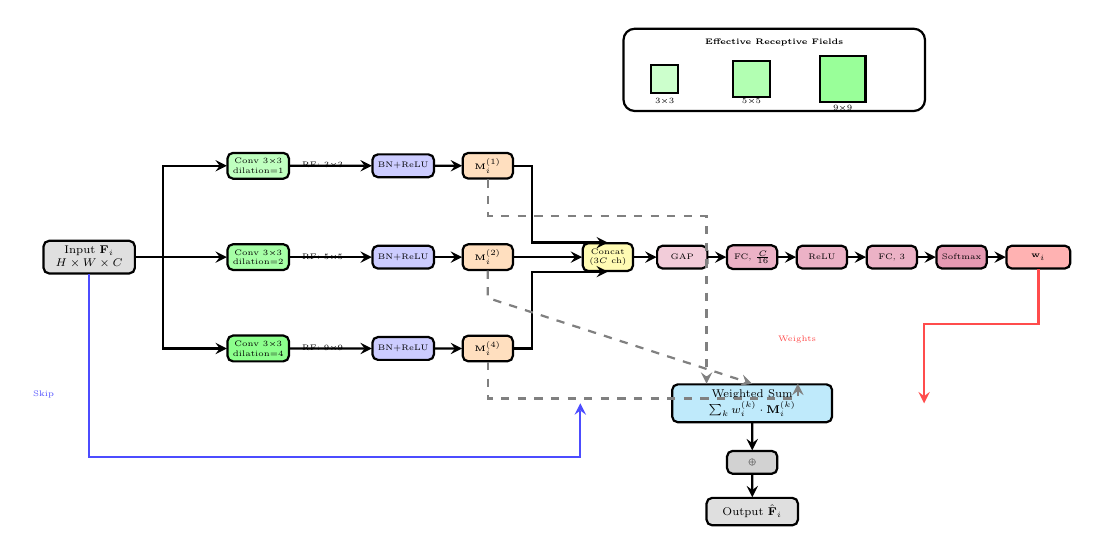
\begin{tikzpicture}[
    scale=0.58,
    transform shape,
    box/.style={draw, thick, rounded corners=2pt, minimum height=0.6cm, minimum width=1.3cm, align=center, font=\scriptsize},
    smallbox/.style={draw, thick, rounded corners=2pt, minimum height=0.5cm, minimum width=1.1cm, align=center, font=\tiny},
    arrow/.style={->, thick, >=stealth}
]

% Input feature - left side
\node[box, fill=gray!25, minimum width=2cm] (input) at (0,0) {Input $\mathbf{F}_i$\\$H \times W \times C$};

% Three parallel branches - clearly separated vertically
\node[smallbox, fill=green!25, right=2cm of input, yshift=2cm] (conv1) {Conv 3×3\\dilation=1};
\node[smallbox, fill=green!35, right=2cm of input, yshift=0cm] (conv2) {Conv 3×3\\dilation=2};
\node[smallbox, fill=green!45, right=2cm of input, yshift=-2cm] (conv4) {Conv 3×3\\dilation=4};

% RF labels - positioned to the right
\node[font=\tiny, fill=white, right=0.15cm of conv1] {RF: 3×3};
\node[font=\tiny, fill=white, right=0.15cm of conv2] {RF: 5×5};
\node[font=\tiny, fill=white, right=0.15cm of conv4] {RF: 9×9};

% BN + ReLU
\node[smallbox, fill=blue!20, right=1.8cm of conv1] (bn1) {BN+ReLU};
\node[smallbox, fill=blue!20, right=1.8cm of conv2] (bn2) {BN+ReLU};
\node[smallbox, fill=blue!20, right=1.8cm of conv4] (bn4) {BN+ReLU};

% Multi-scale features
\node[smallbox, fill=orange!25, right=0.6cm of bn1] (m1) {$\mathbf{M}_i^{(1)}$};
\node[smallbox, fill=orange!25, right=0.6cm of bn2] (m2) {$\mathbf{M}_i^{(2)}$};
\node[smallbox, fill=orange!25, right=0.6cm of bn4] (m4) {$\mathbf{M}_i^{(4)}$};

% Input arrows - fan out cleanly
\draw[arrow] (input.east) -- ++(0.6,0) |- (conv1.west);
\draw[arrow] (input.east) -- ++(0.6,0) -- (conv2.west);
\draw[arrow] (input.east) -- ++(0.6,0) |- (conv4.west);

% Conv to BN arrows
\draw[arrow] (conv1) -- (bn1);
\draw[arrow] (conv2) -- (bn2);
\draw[arrow] (conv4) -- (bn4);

% BN to M arrows
\draw[arrow] (bn1) -- (m1);
\draw[arrow] (bn2) -- (m2);
\draw[arrow] (bn4) -- (m4);

% Concatenate for weight learning
\node[smallbox, fill=yellow!30, right=1.5cm of m2] (cat) {Concat\\($3C$ ch)};

\draw[arrow] (m1.east) -- ++(0.4,0) |- (cat.north);
\draw[arrow] (m2.east) -- (cat.west);
\draw[arrow] (m4.east) -- ++(0.4,0) |- (cat.south);

% Weight learning branch - horizontal
\node[smallbox, fill=purple!20, right=0.5cm of cat] (gap) {GAP};
\node[smallbox, fill=purple!30, right=0.4cm of gap] (fc1) {FC, $\frac{C}{16}$};
\node[smallbox, fill=purple!30, right=0.4cm of fc1] (relu) {ReLU};
\node[smallbox, fill=purple!30, right=0.4cm of relu] (fc2) {FC, 3};
\node[smallbox, fill=purple!40, right=0.4cm of fc2] (sm) {Softmax};
\node[smallbox, fill=red!30, right=0.4cm of sm, minimum width=1.4cm] (w) {$\mathbf{w}_i$};

\draw[arrow] (cat) -- (gap);
\draw[arrow] (gap) -- (fc1);
\draw[arrow] (fc1) -- (relu);
\draw[arrow] (relu) -- (fc2);
\draw[arrow] (fc2) -- (sm);
\draw[arrow] (sm) -- (w);

% Weighted sum block - positioned below
\node[box, fill=cyan!25, below=2.5cm of fc1, minimum width=3.5cm] (wsum) {Weighted Sum\\$\sum_k w_i^{(k)} \cdot \mathbf{M}_i^{(k)}$};

% Connect features to weighted sum with clean routing
\draw[arrow, dashed, gray] (m1.south) -- ++(0,-0.8) -| ([xshift=-1cm]wsum.north);
\draw[arrow, dashed, gray] (m2.south) -- ++(0,-0.6) -- ([xshift=0cm]wsum.north);
\draw[arrow, dashed, gray] (m4.south) -- ++(0,-0.8) -| ([xshift=1cm]wsum.north);

% Weight connection - clean vertical then horizontal
\draw[arrow, red!70, thick] (w.south) -- ++(0,-1.2) -| ([xshift=2cm]wsum.east);
\node[font=\tiny, red!70, fill=white] at (15.5,-1.8) {Weights};

% Skip connection from input - clean routing
\draw[arrow, blue!70, thick] (input.south) -- ++(0,-4) -| ([xshift=-2cm]wsum.west);
\node[font=\tiny, blue!70, fill=white] at (-1,-3) {Skip};

% Addition and output
\node[smallbox, fill=gray!35, below=0.6cm of wsum] (add) {$\oplus$};
\node[box, fill=gray!25, below=0.5cm of add, minimum width=2cm] (output) {Output $\hat{\mathbf{F}}_i$};

\draw[arrow] (wsum) -- (add);
\draw[arrow] (add) -- (output);

% Receptive field illustration - top right corner
\begin{scope}[shift={(12,3.5)}]
\draw[thick, rounded corners, fill=white] (-0.3,-0.3) rectangle (6.3,1.5);
\node[font=\tiny\bfseries] at (3,1.2) {Effective Receptive Fields};
\draw[thick, fill=green!20] (0.3,0.1) rectangle (0.9,0.7);
\node[font=\tiny] at (0.6,-0.1) {3×3};
\draw[thick, fill=green!30] (2.1,0) rectangle (2.9,0.8);
\node[font=\tiny] at (2.5,-0.1) {5×5};
\draw[thick, fill=green!40] (4.0,-0.1) rectangle (5.0,0.9);
\node[font=\tiny] at (4.5,-0.25) {9×9};
\end{scope}

\end{tikzpicture}
\caption{Detailed architecture of the Adaptive Multi-Scale Module (AMSM). Input features $\mathbf{F}_i$ are processed through three parallel 3×3 dilated convolution branches with dilation rates $r \in \{1, 2, 4\}$, producing effective receptive fields of 3×3, 5×5, and 9×9 respectively. Adaptive fusion weights $\mathbf{w}_i = [w^{(1)}, w^{(2)}, w^{(4)}]$ are learned through global average pooling (GAP) and a two-layer fully-connected network with softmax normalization. The weighted multi-scale features are combined with a skip connection from the input, enabling the module to learn scale-adaptive refinements. RF: receptive field; BN: batch normalization.}
\label{fig:amsm}
\end{figure}

For each feature map $\mathbf{F}_i$, AMSM applies three parallel 3$\times$3 dilated convolutions with dilation rates $r \in \{1, 2, 4\}$:
\begin{equation}
\mathbf{M}_i^{(r)} = \text{BN}(\text{ReLU}(\text{Conv}_{3 \times 3}^{d=r}(\mathbf{F}_i)))
\label{eq:dilated}
\end{equation}
where $\text{Conv}_{3 \times 3}^{d=r}$ denotes a 3$\times$3 convolution with dilation rate $r$, BN is batch normalization, and ReLU is the rectified linear unit activation. The effective receptive field sizes are 3$\times$3, 5$\times$5, and 9$\times$9 for dilation rates 1, 2, and 4 respectively, computed as $(k-1) \times d + 1$ where $k=3$ is kernel size.

Rather than fixed fusion weights, we learn input-adaptive weights through a lightweight channel attention mechanism:
\begin{equation}
\mathbf{w}_i = \text{Softmax}(\mathbf{W}_2 \cdot \text{ReLU}(\mathbf{W}_1 \cdot \text{GAP}([\mathbf{M}_i^{(1)}; \mathbf{M}_i^{(2)}; \mathbf{M}_i^{(4)}])))
\label{eq:fusion}
\end{equation}
where GAP denotes global average pooling collapsing spatial dimensions, $[\cdot;\cdot]$ is channel-wise concatenation producing a $3C$-dimensional vector, and $\mathbf{W}_1 \in \mathbb{R}^{(C/16) \times 3C}$, $\mathbf{W}_2 \in \mathbb{R}^{3 \times (C/16)}$ are learnable projection matrices. The reduction ratio of 16 balances expressiveness and parameter efficiency.

The softmax ensures $\sum_k w_i^{(k)} = 1$, creating a convex combination of multi-scale features. The enhanced feature map combines weighted features with residual preservation:
\begin{equation}
\hat{\mathbf{F}}_i = \sum_{k \in \{1,2,4\}} w_i^{(k)} \mathbf{M}_i^{(r_k)} + \mathbf{F}_i
\label{eq:amsm_output}
\end{equation}

The residual connection ensures gradient flow during training and allows the module to learn refinements rather than complete feature transformations.

\subsection*{Dual Attention Module (DAM)}

Brain MRI volumes contain extensive normal anatomical content that dominates image statistics but provides no diagnostic value. DAM implements sequential channel-then-spatial attention\cite{woo2018cbam} to emphasize tumor-relevant features while suppressing background noise (Fig.~\ref{fig:dam}).

% DAM detailed diagram
\begin{figure}[ht]
\centering
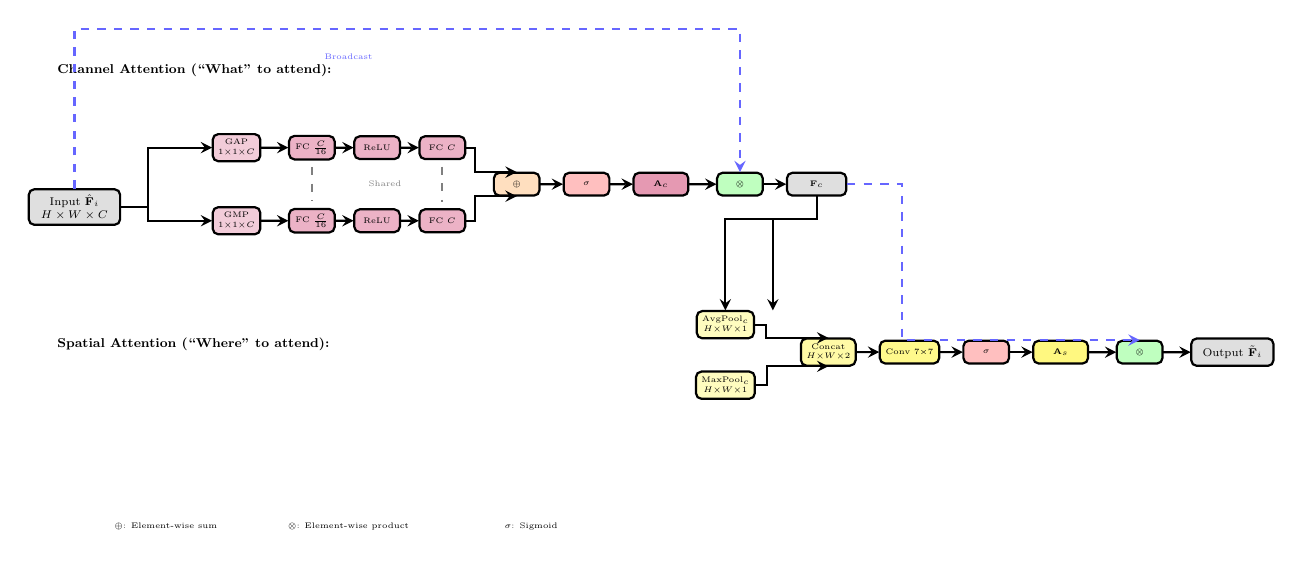
\begin{tikzpicture}[
    scale=0.58,
    transform shape,
    box/.style={draw, thick, rounded corners=2pt, minimum height=0.6cm, minimum width=1.3cm, align=center, font=\scriptsize},
    smallbox/.style={draw, thick, rounded corners=2pt, minimum height=0.5cm, minimum width=1cm, align=center, font=\tiny},
    arrow/.style={->, thick, >=stealth}
]

% Input
\node[box, fill=gray!25, minimum width=2cm] (input) at (0,0) {Input $\hat{\mathbf{F}}_i$\\$H \times W \times C$};

% CHANNEL ATTENTION SECTION - Title
\node[font=\footnotesize\bfseries, anchor=west] at (-0.5,3) {Channel Attention (``What'' to attend):};

% Parallel pooling operations - clearly separated
\node[smallbox, fill=purple!20, right=2cm of input, yshift=1.3cm] (gap) {GAP\\$1{\times}1{\times}C$};
\node[smallbox, fill=purple!20, right=2cm of input, yshift=-0.3cm] (gmp) {GMP\\$1{\times}1{\times}C$};

\draw[arrow] (input.east) -- ++(0.6,0) |- (gap.west);
\draw[arrow] (input.east) -- ++(0.6,0) |- (gmp.west);

% Shared MLP - top path
\node[smallbox, fill=purple!30, right=0.6cm of gap] (fc1a) {FC $\frac{C}{16}$};
\node[smallbox, fill=purple!30, right=0.4cm of fc1a] (relua) {ReLU};
\node[smallbox, fill=purple!30, right=0.4cm of relua] (fc2a) {FC $C$};

% Shared MLP - bottom path
\node[smallbox, fill=purple!30, right=0.6cm of gmp] (fc1b) {FC $\frac{C}{16}$};
\node[smallbox, fill=purple!30, right=0.4cm of fc1b] (relub) {ReLU};
\node[smallbox, fill=purple!30, right=0.4cm of relub] (fc2b) {FC $C$};

\draw[arrow] (gap) -- (fc1a);
\draw[arrow] (fc1a) -- (relua);
\draw[arrow] (relua) -- (fc2a);
\draw[arrow] (gmp) -- (fc1b);
\draw[arrow] (fc1b) -- (relub);
\draw[arrow] (relub) -- (fc2b);

% Shared weights annotation - dashed lines
\draw[dashed, gray, thick] ([yshift=-0.15cm]fc1a.south) -- ([yshift=0.15cm]fc1b.north);
\draw[dashed, gray, thick] ([yshift=-0.15cm]fc2a.south) -- ([yshift=0.15cm]fc2b.north);
\node[font=\tiny, gray, fill=white] at (6.8, 0.5) {Shared};

% Add and sigmoid for channel attention
\node[smallbox, fill=orange!25, right=0.6cm of fc2a, yshift=-0.8cm] (add1) {$\oplus$};
\node[smallbox, fill=red!25, right=0.5cm of add1] (sig1) {$\sigma$};
\node[smallbox, fill=purple!40, right=0.5cm of sig1, minimum width=1.2cm] (ac) {$\mathbf{A}_c$};

\draw[arrow] (fc2a.east) -- ++(0.2,0) |- (add1.north);
\draw[arrow] (fc2b.east) -- ++(0.2,0) |- (add1.south);
\draw[arrow] (add1) -- (sig1);
\draw[arrow] (sig1) -- (ac);

% Channel-refined features
\node[smallbox, fill=green!25, right=0.6cm of ac] (mul1) {$\otimes$};
\node[smallbox, fill=gray!25, right=0.5cm of mul1, minimum width=1.3cm] (fc) {$\mathbf{F}_c$};

\draw[arrow] (ac) -- (mul1);
\draw[arrow, dashed, blue!60] (input.north) -- ++(0,3.5) -| (mul1.north);
\node[font=\tiny, blue!60, fill=white] at (6,3.3) {Broadcast};
\draw[arrow] (mul1) -- (fc);

% SPATIAL ATTENTION SECTION - Title
\node[font=\footnotesize\bfseries, anchor=west] at (-0.5,-3) {Spatial Attention (``Where'' to attend):};

% Channel-wise pooling - positioned below
\node[smallbox, fill=yellow!25, below=2.5cm of fc, xshift=-2cm] (avgpc) {AvgPool$_c$\\$H{\times}W{\times}1$};
\node[smallbox, fill=yellow!25, below=0.7cm of avgpc] (maxpc) {MaxPool$_c$\\$H{\times}W{\times}1$};

\draw[arrow] (fc.south) -- ++(0,-0.5) -| (avgpc.north);
\draw[arrow] (fc.south) -- ++(0,-0.5) -| ([xshift=0.4cm]avgpc.north east);

% Concat and conv for spatial
\node[smallbox, fill=yellow!35, right=1cm of avgpc, yshift=-0.6cm] (cat2) {Concat\\$H{\times}W{\times}2$};
\node[smallbox, fill=yellow!45, right=0.5cm of cat2, minimum width=1.3cm] (conv7) {Conv 7×7};
\node[smallbox, fill=red!25, right=0.5cm of conv7] (sig2) {$\sigma$};
\node[smallbox, fill=yellow!50, right=0.5cm of sig2, minimum width=1.2cm] (as) {$\mathbf{A}_s$};

\draw[arrow] (avgpc.east) -- ++(0.25,0) |- (cat2.north);
\draw[arrow] (maxpc.east) -- ++(0.25,0) |- (cat2.south);
\draw[arrow] (cat2) -- (conv7);
\draw[arrow] (conv7) -- (sig2);
\draw[arrow] (sig2) -- (as);

% Final multiplication
\node[smallbox, fill=green!25, right=0.6cm of as] (mul2) {$\otimes$};
\node[box, fill=gray!25, right=0.6cm of mul2, minimum width=1.8cm] (output) {Output $\tilde{\mathbf{F}}_i$};

\draw[arrow] (as) -- (mul2);
\draw[arrow, dashed, blue!60] (fc.east) -- ++(1.2,0) |- (mul2.north);
\draw[arrow] (mul2) -- (output);

% Legend - bottom
\begin{scope}[shift={(2,-7)}]
\node[font=\tiny, fill=white] at (0,0) {$\oplus$: Element-wise sum};
\node[font=\tiny, fill=white] at (4,0) {$\otimes$: Element-wise product};
\node[font=\tiny, fill=white] at (8,0) {$\sigma$: Sigmoid};
\end{scope}

\end{tikzpicture}
\caption{Detailed architecture of the Dual Attention Module (DAM). Channel attention (top) addresses ``what'' features are informative by recalibrating channel responses through parallel global average pooling (GAP) and global max pooling (GMP), followed by a shared two-layer MLP with bottleneck reduction (ratio 16). Spatial attention (bottom) addresses ``where'' to focus by computing channel-wise pooling statistics concatenated and processed through a 7×7 convolution. Sequential application (channel → spatial) enables feature refinement through ``what'' followed by ``where'' reasoning.}
\label{fig:dam}
\end{figure}

\textbf{Channel Attention} identifies ``what'' features are most informative by recalibrating channel-wise responses:
\begin{equation}
\mathbf{A}_c = \sigma(\text{MLP}(\text{GAP}(\hat{\mathbf{F}}_i)) + \text{MLP}(\text{GMP}(\hat{\mathbf{F}}_i)))
\label{eq:channel_attn}
\end{equation}
where GAP and GMP denote global average and max pooling respectively (collapsing $H \times W$ to $1 \times 1$), MLP is a shared two-layer bottleneck network, and $\sigma$ is the sigmoid activation. Using both pooling operations captures complementary channel statistics: average pooling represents typical activation magnitude while max pooling captures salient responses.

The shared MLP has the form:
\begin{equation}
\text{MLP}(\mathbf{x}) = \mathbf{W}_2(\text{ReLU}(\mathbf{W}_1 \mathbf{x}))
\end{equation}
where $\mathbf{W}_1 \in \mathbb{R}^{(C/16) \times C}$ reduces dimensionality and $\mathbf{W}_2 \in \mathbb{R}^{C \times (C/16)}$ projects back. Weight sharing between the two pooling pathways reduces parameters and enables information exchange.

The channel-refined features are computed through element-wise multiplication with broadcasting:
\begin{equation}
\mathbf{F}_c = \hat{\mathbf{F}}_i \odot \mathbf{A}_c
\end{equation}
where $\odot$ denotes element-wise multiplication and $\mathbf{A}_c \in \mathbb{R}^{1 \times 1 \times C}$ is broadcast across spatial dimensions.

\textbf{Spatial Attention} identifies ``where'' to focus by generating a 2D attention map highlighting discriminative regions:
\begin{equation}
\mathbf{A}_s = \sigma(\text{Conv}_{7 \times 7}([\text{AvgPool}_c(\mathbf{F}_c); \text{MaxPool}_c(\mathbf{F}_c)]))
\label{eq:spatial_attn}
\end{equation}
where $\text{AvgPool}_c$ and $\text{MaxPool}_c$ are channel-wise pooling operations producing $H \times W \times 1$ feature maps. Concatenation yields a 2-channel input to the 7$\times$7 convolution, which captures spatial relationships at an appropriate scale for tumor localization. Padding of 3 preserves spatial dimensions.

The final refined features combine channel and spatial attention:
\begin{equation}
\tilde{\mathbf{F}}_i = \mathbf{F}_c \odot \mathbf{A}_s
\end{equation}

Sequential channel-then-spatial attention has been empirically shown\cite{woo2018cbam} to outperform parallel application by first selecting relevant feature channels before spatially localizing within those channels.

\subsection*{Multi-scale feature aggregation}

Features from all three hierarchical scales are aggregated for final classification. Each refined feature map $\tilde{\mathbf{F}}_i$ undergoes global average pooling to produce fixed-length descriptors independent of spatial dimensions:
\begin{equation}
\mathbf{g}_i = \text{GAP}(\tilde{\mathbf{F}}_i) = \frac{1}{H_i \times W_i} \sum_{h,w} \tilde{\mathbf{F}}_i[h, w, :] \in \mathbb{R}^{C_i}
\end{equation}
yielding $\mathbf{g}_1 \in \mathbb{R}^{48}$ (fine-scale textures), $\mathbf{g}_2 \in \mathbb{R}^{136}$ (mid-level structures), and $\mathbf{g}_3 \in \mathbb{R}^{384}$ (semantic concepts).

These descriptors are concatenated to form the final feature representation:
\begin{equation}
\mathbf{g} = [\mathbf{g}_1; \mathbf{g}_2; \mathbf{g}_3] \in \mathbb{R}^{568}
\end{equation}

This multi-scale aggregation preserves information across all abstraction levels, from fine-grained tumor textures to high-level categorical semantics.

\subsection*{Evidential deep learning classification head}

Standard neural network classifiers use softmax to produce point estimates of class probabilities, precluding meaningful uncertainty quantification. HSANet employs evidential deep learning\cite{sensoy2018evidential}, which places a Dirichlet prior over class probabilities, enabling principled uncertainty estimation from a single forward pass (Fig.~\ref{fig:edl}).

% EDL diagram
\begin{figure}[ht]
\centering
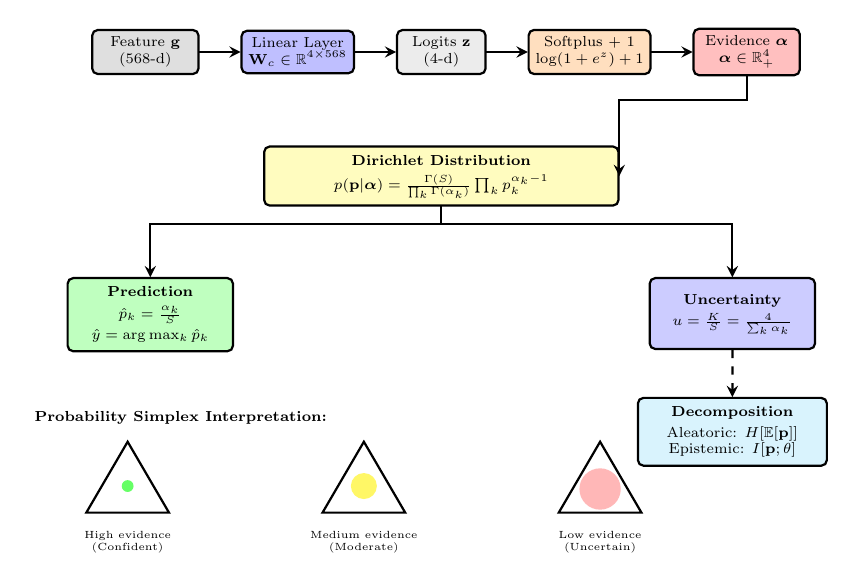
\begin{tikzpicture}[
    scale=0.75,
    transform shape,
    box/.style={draw, thick, rounded corners=2pt, minimum height=0.7cm, align=center, font=\scriptsize},
    smallbox/.style={draw, thick, rounded corners=2pt, minimum height=0.6cm, align=center, font=\tiny},
    arrow/.style={->, thick, >=stealth},
    node distance=0.6cm
]

% ========== TOP ROW: Processing Pipeline ==========
% Feature input
\node[box, fill=gray!25, minimum width=1.8cm] (feat) at (0,0) {Feature $\mathbf{g}$\\(568-d)};

% FC layer
\node[box, fill=blue!25, minimum width=1.8cm, right=0.7cm of feat] (fc) {Linear Layer\\$\mathbf{W}_c \in \mathbb{R}^{4 \times 568}$};

% Logits
\node[box, fill=gray!15, minimum width=1.5cm, right=0.7cm of fc] (z) {Logits $\mathbf{z}$\\(4-d)};

% Softplus
\node[box, fill=orange!25, minimum width=2cm, right=0.7cm of z] (sp) {Softplus + 1\\$\log(1+e^z) + 1$};

% Evidence/Alpha
\node[box, fill=red!25, minimum width=1.8cm, right=0.7cm of sp] (alpha) {Evidence $\boldsymbol{\alpha}$\\$\boldsymbol{\alpha} \in \mathbb{R}^4_+$};

% Arrows for top row
\draw[arrow] (feat) -- (fc);
\draw[arrow] (fc) -- (z);
\draw[arrow] (z) -- (sp);
\draw[arrow] (sp) -- (alpha);

% ========== MIDDLE ROW: Dirichlet Distribution ==========
\node[box, fill=yellow!25, minimum width=6cm, minimum height=1cm, below=1.2cm of z] (dir) {%
    \begin{tabular}{c}
    \textbf{Dirichlet Distribution}\\[2pt]
    $p(\mathbf{p}|\boldsymbol{\alpha}) = \frac{\Gamma(S)}{\prod_k \Gamma(\alpha_k)} \prod_k p_k^{\alpha_k-1}$
    \end{tabular}};

% Arrow from alpha to Dirichlet
\draw[arrow] (alpha.south) -- ++(0,-0.4) -| (dir.east);

% ========== BOTTOM ROW: Outputs ==========
% Prediction box
\node[box, fill=green!25, minimum width=2.8cm, minimum height=1.2cm, below left=1.2cm and 0.5cm of dir] (prob) {%
    \begin{tabular}{c}
    \textbf{Prediction}\\[2pt]
    $\hat{p}_k = \frac{\alpha_k}{S}$\\[2pt]
    $\hat{y} = \arg\max_k \hat{p}_k$
    \end{tabular}};

% Uncertainty box
\node[box, fill=blue!20, minimum width=2.8cm, minimum height=1.2cm, below right=1.2cm and 0.5cm of dir] (unc) {%
    \begin{tabular}{c}
    \textbf{Uncertainty}\\[2pt]
    $u = \frac{K}{S} = \frac{4}{\sum_k \alpha_k}$
    \end{tabular}};

% Arrows to outputs
\draw[arrow] (dir.south) -- ++(0,-0.3) -| (prob.north);
\draw[arrow] (dir.south) -- ++(0,-0.3) -| (unc.north);

% ========== UNCERTAINTY DECOMPOSITION ==========
\node[box, fill=cyan!15, minimum width=3.2cm, minimum height=1cm, below=0.8cm of unc] (decomp) {%
    \begin{tabular}{c}
    \textbf{Decomposition}\\[2pt]
    Aleatoric: $H[\mathbb{E}[\mathbf{p}]]$\\
    Epistemic: $I[\mathbf{p}; \theta]$
    \end{tabular}};

\draw[arrow, dashed] (unc) -- (decomp);

% ========== SIMPLEX INTERPRETATION (Bottom) ==========
\node[font=\scriptsize\bfseries, anchor=west] at (-2, -6.2) {Probability Simplex Interpretation:};

% High evidence simplex
\begin{scope}[shift={(-1,-7.8)}]
    \draw[thick, fill=white] (0,0) -- (1.4,0) -- (0.7,1.2) -- cycle;
    \fill[green!60] (0.7,0.45) circle (0.1);
    \node[font=\tiny, align=center] at (0.7,-0.5) {High evidence\\(Confident)};
\end{scope}

% Medium evidence simplex
\begin{scope}[shift={(3,-7.8)}]
    \draw[thick, fill=white] (0,0) -- (1.4,0) -- (0.7,1.2) -- cycle;
    \fill[yellow!60] (0.7,0.45) circle (0.22);
    \node[font=\tiny, align=center] at (0.7,-0.5) {Medium evidence\\(Moderate)};
\end{scope}

% Low evidence simplex
\begin{scope}[shift={(7,-7.8)}]
    \draw[thick, fill=white] (0,0) -- (1.4,0) -- (0.7,1.2) -- cycle;
    \fill[red!40, opacity=0.7] (0.7,0.4) circle (0.35);
    \node[font=\tiny, align=center] at (0.7,-0.5) {Low evidence\\(Uncertain)};
\end{scope}

\end{tikzpicture}
\caption{Evidential deep learning classification head. The 568-dimensional feature vector is projected to 4 logits via a linear layer. Softplus activation plus 1 ensures positive Dirichlet concentration parameters $\boldsymbol{\alpha} \geq 1$. The Dirichlet distribution over class probabilities yields predictions via its mean and uncertainty via the inverse of total evidence $S$. Bottom: geometric interpretation on the probability simplex---high evidence produces concentrated distributions (confident predictions), low evidence produces spread distributions (uncertain predictions). Uncertainty decomposes into aleatoric (inherent data ambiguity) and epistemic (model knowledge gaps) components.}
\label{fig:edl}
\end{figure}

The network outputs Dirichlet concentration parameters through a non-negative transformation:
\begin{equation}
\boldsymbol{\alpha} = \text{Softplus}(\mathbf{z}) + 1 = \log(1 + e^{\mathbf{z}}) + 1
\label{eq:alpha}
\end{equation}
where $\mathbf{z} = \mathbf{W}_c \mathbf{g} + \mathbf{b}_c$ are the classifier logits ($\mathbf{W}_c \in \mathbb{R}^{4 \times 568}$, $\mathbf{b}_c \in \mathbb{R}^4$). The softplus function ensures positive evidence, and adding 1 guarantees $\alpha_k \geq 1$ for valid Dirichlet parameters (uniform prior when $\boldsymbol{\alpha} = \mathbf{1}$).

The Dirichlet distribution $\text{Dir}(\mathbf{p} | \boldsymbol{\alpha})$ has probability density function:
\begin{equation}
p(\mathbf{p} | \boldsymbol{\alpha}) = \frac{\Gamma(S)}{\prod_{k=1}^{K} \Gamma(\alpha_k)} \prod_{k=1}^{K} p_k^{\alpha_k - 1}
\end{equation}
where $S = \sum_{k=1}^{K} \alpha_k$ is the Dirichlet strength (total evidence), $K=4$ is the number of classes, and $\Gamma(\cdot)$ is the gamma function.

\textbf{Prediction:} Class probabilities are computed as the Dirichlet mean:
\begin{equation}
\hat{p}_k = \mathbb{E}[p_k | \boldsymbol{\alpha}] = \frac{\alpha_k}{S}
\end{equation}
The predicted class is $\hat{y} = \arg\max_k \hat{p}_k$.

\textbf{Uncertainty:} Total predictive uncertainty is quantified as:
\begin{equation}
u = \frac{K}{S} = \frac{4}{\sum_{k=1}^{4} \alpha_k}
\end{equation}
Higher values indicate lower total evidence and thus higher uncertainty. This uncertainty naturally decomposes into:

\begin{itemize}
\item \textbf{Aleatoric uncertainty} (data uncertainty): Quantified by the entropy of the expected distribution:
\begin{equation}
u_{\text{aleatoric}} = H[\mathbb{E}[\mathbf{p} | \boldsymbol{\alpha}]] = -\sum_k \hat{p}_k \log \hat{p}_k
\end{equation}
This captures inherent class overlap where imaging characteristics are ambiguous between categories.

\item \textbf{Epistemic uncertainty} (model uncertainty): Quantified by the mutual information between predictions and parameters:
\begin{equation}
u_{\text{epistemic}} = I[\mathbf{p}; \theta | \mathbf{x}] = H[\mathbb{E}[\mathbf{p}]] - \mathbb{E}[H[\mathbf{p}]]
\end{equation}
This captures model knowledge gaps, flagging inputs dissimilar to training data.
\end{itemize}

\subsection*{Loss function and training objective}

The training objective combines three complementary loss terms designed to encourage correct classification, handle class imbalance, and prevent overconfident incorrect predictions (Fig.~\ref{fig:training}):

\textbf{1. Evidence-weighted Cross-Entropy Loss:}
\begin{equation}
\mathcal{L}_{\text{CE}} = \sum_{k=1}^{K} y_k \left( \psi(S) - \psi(\alpha_k) \right)
\end{equation}
where $\mathbf{y} = [y_1, ..., y_K]$ is the one-hot encoded ground truth label and $\psi(\cdot)$ is the digamma function (derivative of log-gamma). This loss encourages the model to accumulate evidence for the correct class while being derived from the negative log-likelihood of the Dirichlet-Multinomial model.

\textbf{2. Focal Loss for Class Imbalance:}
\begin{equation}
\mathcal{L}_{\text{focal}} = -\sum_{k=1}^{K} y_k (1 - \hat{p}_k)^\gamma \log(\hat{p}_k)
\label{eq:focal}
\end{equation}
with focusing parameter $\gamma = 2$. Focal loss\cite{lin2017focal} down-weights well-classified examples (high $\hat{p}_k$) to focus learning on hard cases, mitigating class imbalance effects without explicit sample weighting.

\textbf{3. KL Divergence Regularization:}
\begin{equation}
\mathcal{L}_{\text{KL}} = \text{KL}\left[ \text{Dir}(\mathbf{p} | \tilde{\boldsymbol{\alpha}}) \| \text{Dir}(\mathbf{p} | \mathbf{1}) \right]
\end{equation}
where $\tilde{\boldsymbol{\alpha}} = \mathbf{y} + (1 - \mathbf{y}) \odot \boldsymbol{\alpha}$ removes evidence for the correct class. This penalizes evidence for incorrect classes, preventing the model from being confidently wrong. The KL divergence from a uniform Dirichlet prior has closed form:
\begin{equation}
\text{KL}[\text{Dir}(\mathbf{p}|\tilde{\boldsymbol{\alpha}}) \| \text{Dir}(\mathbf{p}|\mathbf{1})] = \log \frac{\Gamma(\tilde{S})}{\Gamma(K)} + \sum_k \left[ (\tilde{\alpha}_k - 1)(\psi(\tilde{\alpha}_k) - \psi(\tilde{S})) \right]
\end{equation}

The total loss combines these terms:
\begin{equation}
\mathcal{L} = \lambda_1 \mathcal{L}_{\text{CE}} + \lambda_2 \mathcal{L}_{\text{focal}} + \lambda_3 \mathcal{L}_{\text{KL}}
\end{equation}
with weights $\lambda_1 = 0.5$, $\lambda_2 = 0.3$, $\lambda_3 = 0.2$ determined through validation set tuning.

To prevent premature regularization before the model learns discriminative features, the KL weight is annealed:
\begin{equation}
\lambda_3^{(t)} = \min\left(1, \frac{t}{T_{\text{anneal}}}\right) \cdot \lambda_3
\end{equation}
ramping from 0 to full strength over $T_{\text{anneal}} = 10$ epochs.

% Training pipeline diagram
\begin{figure}[ht]
\centering
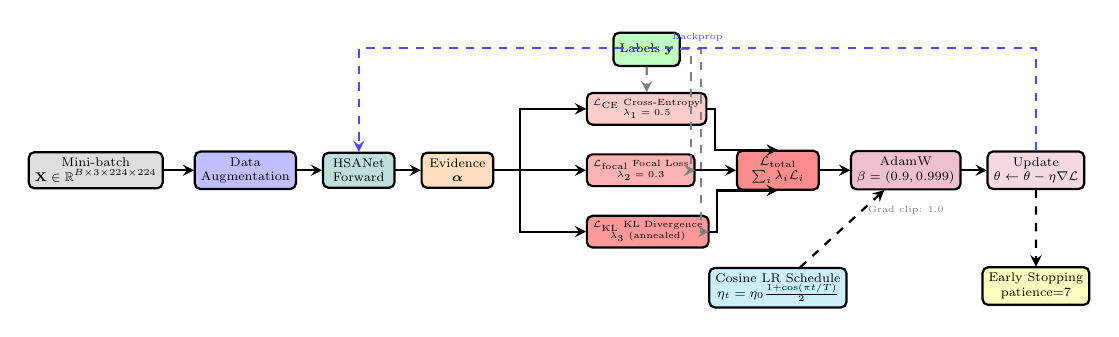
\begin{tikzpicture}[
    scale=0.65,
    transform shape,
    box/.style={draw, thick, rounded corners=2pt, minimum height=0.65cm, align=center, font=\scriptsize},
    lossbox/.style={draw, thick, rounded corners=2pt, minimum height=0.55cm, align=center, font=\tiny},
    arrow/.style={->, thick, >=stealth},
    node distance=0.5cm
]

% ========== DATA FLOW (LEFT SECTION) ==========
\node[box, fill=gray!25, minimum width=2cm] (batch) at (0,0) {Mini-batch\\$\mathbf{X} \in \mathbb{R}^{B \times 3 \times 224 \times 224}$};
\node[box, fill=blue!25, minimum width=1.4cm, right=0.6cm of batch] (aug) {Data\\Augmentation};
\node[box, fill=teal!25, minimum width=1.4cm, right=0.5cm of aug] (model) {HSANet\\Forward};
\node[box, fill=orange!25, minimum width=1.4cm, right=0.5cm of model] (alpha) {Evidence\\$\boldsymbol{\alpha}$};

\draw[arrow] (batch) -- (aug);
\draw[arrow] (aug) -- (model);
\draw[arrow] (model) -- (alpha);

% ========== LOSS BRANCHES (MIDDLE SECTION) ==========
% Three loss boxes vertically arranged
\node[lossbox, fill=red!20, minimum width=1.8cm, right=1.8cm of alpha, yshift=1.2cm] (lce) {$\mathcal{L}_{\text{CE}}$ Cross-Entropy\\$\lambda_1=0.5$};
\node[lossbox, fill=red!30, minimum width=1.8cm, right=1.8cm of alpha] (lfocal) {$\mathcal{L}_{\text{focal}}$ Focal Loss\\$\lambda_2=0.3$};
\node[lossbox, fill=red!40, minimum width=1.8cm, right=1.8cm of alpha, yshift=-1.2cm] (lkl) {$\mathcal{L}_{\text{KL}}$ KL Divergence\\$\lambda_3$ (annealed)};

% Arrows from alpha to losses
\draw[arrow] (alpha.east) -- ++(0.5,0) |- (lce.west);
\draw[arrow] (alpha.east) -- ++(0.5,0) -- (lfocal.west);
\draw[arrow] (alpha.east) -- ++(0.5,0) |- (lkl.west);

% Ground truth labels
\node[box, fill=green!25, minimum width=1.2cm, above=0.5cm of lce] (gt) {Labels $\mathbf{y}$};
\draw[arrow, dashed, gray] (gt) -- (lce);
\draw[arrow, dashed, gray] (gt.east) -- ++(0.2,0) |- (lfocal.east);
\draw[arrow, dashed, gray] (gt.east) -- ++(0.4,0) |- (lkl.east);

% ========== TOTAL LOSS (CENTER-RIGHT) ==========
\node[box, fill=red!45, minimum width=1.6cm, right=0.8cm of lfocal] (total) {$\mathcal{L}_{\text{total}}$\\$\sum_i \lambda_i \mathcal{L}_i$};

\draw[arrow] (lce.east) -- ++(0.15,0) |- (total.north);
\draw[arrow] (lfocal) -- (total);
\draw[arrow] (lkl.east) -- ++(0.15,0) |- (total.south);

% ========== OPTIMIZER (RIGHT SECTION) ==========
\node[box, fill=purple!25, minimum width=1.5cm, right=0.6cm of total] (opt) {AdamW\\$\beta=(0.9, 0.999)$};
\node[box, fill=purple!15, minimum width=1.6cm, right=0.5cm of opt] (update) {Update\\$\theta \leftarrow \theta - \eta \nabla \mathcal{L}$};

\draw[arrow] (total) -- (opt);
\draw[arrow] (opt) -- (update);

% ========== FEEDBACK LOOP ==========
\draw[arrow, dashed, blue!70, thick] (update.north) -- ++(0,2) -| node[pos=0.25, above, font=\tiny, blue!70] {Backprop} (model.north);

% ========== AUXILIARY COMPONENTS (BOTTOM) ==========
% Learning rate schedule
\node[box, fill=cyan!20, minimum width=2.2cm, below=1.5cm of total] (lr) {Cosine LR Schedule\\$\eta_t = \eta_0 \frac{1+\cos(\pi t/T)}{2}$};
\draw[arrow, dashed] (lr) -- (opt);

% Early stopping
\node[box, fill=yellow!25, minimum width=1.5cm, below=1.5cm of update] (es) {Early Stopping\\patience=7};
\draw[arrow, dashed] (update.south) -- (es);

% Gradient clipping annotation
\node[font=\tiny, gray] at ([yshift=-0.4cm]opt.south) {Grad clip: 1.0};

\end{tikzpicture}
\caption{Complete training pipeline. Mini-batches undergo data augmentation before forward propagation through HSANet. Three loss terms are computed: evidence-weighted cross-entropy, focal loss for class imbalance, and KL divergence regularization (annealed during early training). AdamW optimizer updates parameters with cosine learning rate annealing. Early stopping monitors validation loss with patience of 7 epochs. Gradient clipping (norm 1.0) ensures training stability.}
\label{fig:training}
\end{figure}

\subsection*{Training configuration}

Training employed the following hyperparameters, determined through systematic grid search on a held-out validation set (10\% of training data):

\begin{itemize}
\item \textbf{Optimizer}: AdamW\cite{loshchilov2017decoupled} with $\beta_1 = 0.9$, $\beta_2 = 0.999$, weight decay $10^{-4}$
\item \textbf{Learning rate}: Initial $\eta_0 = 3 \times 10^{-4}$, cosine annealing to $\eta_{\min} = 10^{-6}$
\item \textbf{Backbone learning rate}: $\eta_{\text{backbone}} = \eta_0 / 10$ (10× lower for transfer learning stability)
\item \textbf{Batch size}: 32 (limited by GPU memory)
\item \textbf{Epochs}: Maximum 30 with early stopping (patience 7 epochs)
\item \textbf{Gradient clipping}: Maximum norm 1.0 for training stability
\item \textbf{Random seeds}: Fixed at 42 for full reproducibility
\item \textbf{Backbone freezing}: First 5 epochs to stabilize custom module training
\end{itemize}

The complete training algorithm is presented in Algorithm~\ref{alg:training}.

\begin{algorithm}[ht]
\caption{HSANet Training Procedure}
\label{alg:training}
\begin{algorithmic}[1]
\Require Training set $\mathcal{D}_{\text{train}}$, validation set $\mathcal{D}_{\text{val}}$
\Require Hyperparameters: $\eta_0$, $\lambda_1$, $\lambda_2$, $\lambda_3$, $T_{\text{anneal}}$, $T_{\text{max}}$, patience
\State Initialize EfficientNet-B3 backbone with ImageNet pretrained weights
\State Initialize AMSM, DAM modules with Kaiming initialization
\State Initialize evidential head with Xavier initialization
\State Freeze backbone parameters for first 5 epochs
\State $t \gets 0$; $\text{best\_loss} \gets \infty$; $\text{wait} \gets 0$
\For{epoch $= 1$ to $T_{\text{max}}$}
    \If{epoch $= 6$}
        \State Unfreeze backbone with learning rate $\eta_0 / 10$
    \EndIf
    \State $\lambda_3^{(t)} \gets \min(1, t/T_{\text{anneal}}) \cdot \lambda_3$ \Comment{Anneal KL weight}
    \State $\eta_t \gets \eta_0 \cdot \frac{1 + \cos(\pi \cdot t / T_{\text{max}})}{2}$ \Comment{Cosine LR schedule}
    \For{each mini-batch $(\mathbf{X}, \mathbf{y})$ in $\mathcal{D}_{\text{train}}$}
        \State $\mathbf{X}_{\text{aug}} \gets \text{Augment}(\mathbf{X})$ \Comment{Apply data augmentation}
        \State $\boldsymbol{\alpha} \gets \text{HSANet}(\mathbf{X}_{\text{aug}})$ \Comment{Forward pass}
        \State Compute $\mathcal{L}_{\text{CE}}$, $\mathcal{L}_{\text{focal}}$, $\mathcal{L}_{\text{KL}}$ using Equations (10-12)
        \State $\mathcal{L} \gets \lambda_1 \mathcal{L}_{\text{CE}} + \lambda_2 \mathcal{L}_{\text{focal}} + \lambda_3^{(t)} \mathcal{L}_{\text{KL}}$
        \State $\nabla_\theta \mathcal{L} \gets \text{Backpropagate}(\mathcal{L})$
        \State Clip $\|\nabla_\theta \mathcal{L}\|_2$ to maximum 1.0
        \State $\theta \gets \text{AdamW}(\theta, \nabla_\theta \mathcal{L}, \eta_t)$
    \EndFor
    \State $\mathcal{L}_{\text{val}} \gets \text{Evaluate}(\mathcal{D}_{\text{val}})$
    \If{$\mathcal{L}_{\text{val}} < \text{best\_loss}$}
        \State Save checkpoint; $\text{best\_loss} \gets \mathcal{L}_{\text{val}}$; $\text{wait} \gets 0$
    \Else
        \State $\text{wait} \gets \text{wait} + 1$
    \EndIf
    \If{$\text{wait} \geq \text{patience}$}
        \State \textbf{break} \Comment{Early stopping triggered}
    \EndIf
    \State $t \gets t + 1$
\EndFor
\State \Return Best model checkpoint
\end{algorithmic}
\end{algorithm}

\subsection*{Evaluation metrics}

Classification performance was assessed using standard metrics:
\begin{itemize}
\item \textbf{Accuracy}: $\text{Acc} = \frac{\text{TP} + \text{TN}}{\text{Total}}$
\item \textbf{Precision}: $\text{Prec}_k = \frac{\text{TP}_k}{\text{TP}_k + \text{FP}_k}$ (per-class and macro-averaged)
\item \textbf{Recall/Sensitivity}: $\text{Rec}_k = \frac{\text{TP}_k}{\text{TP}_k + \text{FN}_k}$
\item \textbf{F1-Score}: $\text{F1}_k = \frac{2 \cdot \text{Prec}_k \cdot \text{Rec}_k}{\text{Prec}_k + \text{Rec}_k}$
\item \textbf{Cohen's $\kappa$}: Agreement correcting for chance: $\kappa = \frac{p_o - p_e}{1 - p_e}$
\item \textbf{Matthews Correlation Coefficient}: $\text{MCC} = \frac{\text{TP} \cdot \text{TN} - \text{FP} \cdot \text{FN}}{\sqrt{(\text{TP}+\text{FP})(\text{TP}+\text{FN})(\text{TN}+\text{FP})(\text{TN}+\text{FN})}}$
\item \textbf{AUC-ROC}: Area under ROC curve using one-vs-rest strategy for multiclass
\end{itemize}

Model calibration was evaluated using:
\begin{itemize}
\item \textbf{Expected Calibration Error (ECE)}: $\text{ECE} = \sum_{m=1}^{M} \frac{|B_m|}{n} |\text{acc}(B_m) - \text{conf}(B_m)|$

where predictions are binned into $M=15$ equal-width intervals by confidence, $|B_m|$ is bin size, $\text{acc}(B_m)$ is accuracy within bin, and $\text{conf}(B_m)$ is mean confidence within bin.
\item \textbf{Reliability Diagram}: Visual comparison of confidence vs. accuracy per bin
\end{itemize}

Interpretability was assessed using GradCAM\cite{selvaraju2017grad}, computing gradient-weighted activations from the final convolutional layer:
\begin{equation}
L^c_{\text{GradCAM}} = \text{ReLU}\left(\sum_k \alpha_k^c A^k\right), \quad \alpha_k^c = \frac{1}{Z} \sum_i \sum_j \frac{\partial y^c}{\partial A^k_{ij}}
\end{equation}
where $A^k$ is the $k$-th feature map, $y^c$ is the class score, and $\alpha_k^c$ weights feature map importance.

\subsection*{Statistical analysis}

95\% confidence intervals for accuracy were computed using the Wilson score interval, appropriate for proportions. Five-fold stratified cross-validation assessed model stability, maintaining class proportions across folds. Statistical significance of performance differences was assessed using McNemar's test for paired comparisons. All experiments were repeated with three random seeds (42, 123, 456); reported values are means with standard deviations.

\subsection*{Implementation details}

All experiments were conducted using PyTorch 2.0 with the following computational environment:
\begin{itemize}
\item \textbf{Hardware}: NVIDIA Tesla P100 GPU (16GB VRAM), 30GB system RAM
\item \textbf{Operating System}: Ubuntu 20.04 LTS
\item \textbf{Software}: Python 3.10, PyTorch 2.0.1, CUDA 11.8, cuDNN 8.6
\item \textbf{Key Libraries}: timm 0.9.2 (EfficientNet implementation), scikit-learn 1.3.0, matplotlib 3.7.1, numpy 1.24.3
\end{itemize}

Single-image inference requires 12 milliseconds on P100 GPU (batch size 1), enabling real-time clinical deployment at $>$80 images/second. Training converges in approximately 25 epochs (45 minutes total wall-clock time).

\subsection*{Data availability}

The Brain Tumor MRI Dataset used for training and primary evaluation is publicly available at:\\
\url{https://www.kaggle.com/datasets/masoudnickparvar/brain-tumor-mri-dataset}

The Figshare Brain Tumor Dataset used for external validation is publicly available at:\\
\url{https://figshare.com/articles/dataset/brain_tumor_dataset/1512427}

No restrictions apply to data access for either dataset.

\subsection*{Code availability}

Complete source code for HSANet, including training scripts, evaluation pipelines, cross-dataset validation scripts, pretrained model weights, and documentation, is publicly available at:\\
\url{https://github.com/tarequejosh/hsanet-brain-tumor}

The repository includes:
\begin{itemize}
\item Model architecture implementation (\texttt{hsanet\_model.py})
\item Training pipeline (\texttt{training\_pipeline.py})
\item Cross-dataset validation pipeline (\texttt{cross\_dataset\_validation.py})
\item Figshare dataset preprocessing script (\texttt{convert\_figshare\_dataset.py})
\item Evaluation and visualization scripts
\item Pretrained model checkpoints
\item Requirements specification for environment reproduction
\end{itemize}

\bibliography{references}

\section*{Acknowledgements}

The authors acknowledge the Department of Computer Science and Engineering, Daffodil International University, for providing computational resources. We thank the creators of the Brain Tumor MRI Dataset for making their data publicly available for research purposes. We also acknowledge the developers of PyTorch, EfficientNet, and related open-source tools that made this research possible.

\section*{Author contributions statement}

M.A. conceived the research direction, designed the methodology, and supervised the project. M.T.J.J. developed the software implementation, conducted all experiments, performed data analysis, and wrote the original manuscript draft. M.A.R.J. performed data curation, created visualizations, and contributed to manuscript preparation. M.N.I.I. contributed to experimental validation, literature review, and manuscript revision. All authors reviewed, edited, and approved the final manuscript.

\section*{Additional information}

\textbf{Competing interests:} The authors declare no competing financial or non-financial interests.

\end{document}
